\documentclass[a4paper, 11pt]{article}
\usepackage{verbatim} 
\usepackage{amsmath}
\usepackage{amsfonts}
\usepackage{amssymb}
\usepackage{amsthm}
\usepackage{siunitx}
\sisetup{
    %output-decimal-marker={,}% just uncomment if you want to use comma as the decimal marker!
}
\usepackage{caratula}
\usepackage{listings}
\usepackage[utf8]{inputenc}
\usepackage[spanish, activeacute]{babel}
\usepackage[usenames,dvipsnames]{color}
\usepackage[width=15.5cm, left=3cm, top=2.5cm, height= 24.5cm]{geometry}
\usepackage{graphicx}
%\usepackage{subcaption}
\usepackage[all]{xy}
\usepackage{multicol}
\usepackage{subfig}
\usepackage{algorithm}
\usepackage{algorithmic}
\usepackage{cancel}
\usepackage{array}
\usepackage{float}
\usepackage{xcolor}
\usepackage{color,hyperref}
\setcounter{secnumdepth}{3} %%agrego subsubsection
\usepackage[nottoc,notlot,notlof]{tocbibind}

\newtheorem{lema}{Lema}
\newtheorem{teorema}{Teorema}
\newtheorem{corolario}{Corolario}
\newtheorem*{correctitud}{Correctitud del algoritmo}
\newtheorem*{notacion}{Notación}

\lstset{basicstyle=\small\ttfamily, breaklines=true, breakatwhitespace=true}
\lstset{numbers=left, numberstyle=\scriptsize}
\lstset{
     literate=%
         {á}{{\'a}}1
         {í}{{\'i}}1
         {é}{{\'e}}1
         {ý}{{\'y}}1
         {ú}{{\'u}}1
         {ó}{{\'o}}1
         {ě}{{\v{e}}}1
         {š}{{\v{s}}}1
         {č}{{\v{c}}}1
         {ř}{{\v{r}}}1
         {ž}{{\v{z}}}1
         {ď}{{\v{d}}}1
         {ť}{{\v{t}}}1
         {ñ}{{\~n}}1                
         {ů}{{\r{u}}}1
         {Á}{{\'A}}1
         {Í}{{\'I}}1
         {É}{{\'E}}1
         {Ý}{{\'Y}}1
         {Ú}{{\'U}}1
         {Ó}{{\'O}}1
         {Ě}{{\v{E}}}1
         {Š}{{\v{S}}}1
         {Č}{{\v{C}}}1
         {Ř}{{\v{R}}}1
         {Ž}{{\v{Z}}}1
         {Ď}{{\v{D}}}1
         {Ť}{{\v{T}}}1
         {Ň}{{\v{N}}}1                
         {Ů}{{\r{U}}}1    
}


%%%%%%%%%%%%%% ALGUNAS MACROS %%%%%%%%%%%%%%
% For \url{SOME_URL}, links SOME_URL to the url SOME_URL
\providecommand*\url[1]{\href{#1}{#1}}

\setlength{\parskip}{10pt plus 1pt minus 1pt}
\usepackage{tikz}
\def\checkmark{\tikz\fill[scale=0.4](0,.35) -- (.25,0) -- (1,.7) -- (.25,.15) -- cycle;}

% Same as above, but pretty-prints SOME_URL in teletype fixed-width font
\renewcommand*\url[1]{\href{#1}{\texttt{#1}}}

% Comando para poner el simbolo de Reales
\newcommand{\real}{\hbox{\bf R}}

\providecommand*\code[1]{\texttt{#1}}

%uso: \ponerGrafico{file}{caption}{scale}{label}
\newcommand{\ponerGrafico}[4]
{\begin{figure}[H]
	\centering
	\subfloat{\includegraphics[scale=#3]{#1}}
	\caption{#2} \label{fig:#4}
\end{figure}
}

\renewcommand{\algorithmiccomment}[1]{\hfill #1}

%%%%%%%%%%%%%%%%%%%%%%%%%%%%%%%%%%%%%%%%%%%%

\materia{Algoritmos y Estructuras de Datos III}

\titulo{Trabajo práctico 3}
%\fecha{fecha de entrega}
%\grupo{Nro grupo}
\integrante{Sebastián Fernández Ledesma}{392/06}{sfernandezledesma@gmail.com}
\integrante{Fernando Gasperi Jabalera}{56/09}{fgasperijabalera@gmail.com}
\integrante{Maximiliano Wortman}{892/10}{maxifwortman@gmail.com}
\integrante{Santiago Camacho}{110/09}{santicamacho90@gmail.com}


%\include{templates}

\begin{document}
\pagestyle{myheadings}
\maketitle
%\markboth{Nombre materia}{Nombre TP}

\thispagestyle{empty}
\tableofcontents

%\setcounter{section}{-1}
\newpage
\section{Ejercicio 1}

\begin{displaymath}
	\sum_0^{\infty}laposta de 
\end{displaymath}

\section{Algoritmo exacto}

\subsection{Descripción del algoritmo}
El algoritmo utilizado para obtener la $k$-PMP de un grafo $G$ consiste en construir 
todas las posibles soluciones de manera ordenada para mediante backtracking.
Veamos qué contiene el conjunto de soluciones posibles $S$ asociado a un grafo $G = (V, E)$.
Sea $P_V$ el conjunto con todas las particiones posibles del conjunto $V$:
\begin{displaymath}
  S = \left\{p \quad | \quad p \in P_V \land \left\vert{p}\right\vert \leq k\right\}
\end{displaymath}
Todas las particiones de un conjunto de $n$ elementos se pueden obtener recursivamente. Si contamos
con todas las particiones de $i$ elementos, denominaremos $S_i$ al conjunto que contiene a todas las
particiones de $i$ elementos, entonces podemos generar todas las particiones de $i+1$ elementos simplemente 
tomando cada una de las particiones pertenecientes a $S_i$ y agregando el elemento $i+1$ a cada uno 
de sus subconjuntos. Describimos este procedimiento con un pequeño pseudocódigo:

\begin{algorithm}[H]
\begin{algorithmic}
\caption{Particiones}
  \STATE $S_{i+1}\gets \emptyset$
  \WHILE {$S_i \neq \emptyset$}
    \STATE $s\gets$ sacarUno($S_i$)
    \FOR {$j \gets 0...\left\vert{s}\right\vert$}
      \STATE $nuevoSubconjunto \gets $ dameIesimo($j$, $s$)
      \STATE $nuevoSubconjunto \cup e_{i+1}$
      \STATE $S_{i+1} \cup \left\{ s \setminus \text{dameIesimo(}j\text{, }s\text{)} \cup nuevoSubconjunto \right\}$
    \ENDFOR
  \ENDWHILE
\end{algorithmic}
\end{algorithm}

Se puede ver fácilmente que con este procedimiento efectivamente consideramos todas las particiones
posibles que se pueden obtener con los $n$ vértices de $V$. Sin embargo, estamos considerando muchas
particiones que no es necesario tener en cuenta. Por ejemplo, aquellas que tengan una cantidad de
subconjuntos mayor a $k$.

\subsection{Podas y estrategias}
%\begin{lema}
%\label{lema_ej2}
%acá va el enunciado del lema
%\end{lema}
%\begin{proof}
%  Acá va la demostración.
%\end{proof}

Las podas que le agregamos a nuestro backtracking para reducir el árbol de soluciones son:
\begin{enumerate}
  \item no consideraremos particiones que tengan más de $k$ subconjuntos. Una vez que tenemos
    $k$ subconjuntos en la solución actual no agregamos más ya que la solución no puede tener
    más de $k$ subconjuntos. El costo de esta poda es $O(1)$ porque sólo requiere una comparación
    de tipos primitivos.

  \item no considerar particiones que utilicen menos de $k$ subconjuntos. Si estamos
    buscando la $k$-PMP de $G$, llamémosla $P_{min}$ y la misma utiliza menos de $k$ subconjuntos 
    $|P_{min}| < k$ entonces su peso total necesariamente es nulo $\omega(P_{min}) = 0$ ya que si
    hubiera algún subconjunto $s$ con peso mayor 0 eso indicaría que existe alguna arista $e = (v, u)$ intra-partición
    en ese subconjunto con peso mayor a 0. Por lo tanto, si tomamos a $v$ uno de los extremos de esa
    arista y lo pasamos a un subconjunto $s'$ vacío entonces obtendríamos una nueva partición con un peso
    estrictamente menor al de la mínima lo cual es absurdo.
    En el algoritmo esto se ve reflejado cuando la cantidad de subconjuntos no utilizados es igual a la cantidad 
    de nodos que nos quedan por ubicar $|P_{actual}|-k = |nodosRestantes|$. En ese caso lo que hacemos es agregar los $|nodosRestantes|$
    a cada uno de los subconjuntos todavía no utilizados ya que cualquier partición $P'$ que agregue alguno
    de los $nodosRestantes$ a uno de los subconjuntos ya utilizados necesariamente cumple que 
    $\omega(P') \geq \omega(P_{actual})$ porque $P_{actual}$ no va a tener más aristas intra-partición
    y agregando nodos a conjuntos ya utilizados puede que agreguemos aristas intra-partición o no.
    Esta poda también tiene costo $O(1)$ porque sólo necesita que se comparen la cantidad de subconjuntos
    vacíos con la cantidad de nodos restantes. Ambos valores son conocidos en todo momento del algoritmo.

  \item inicializamos $pesoMinimo = +\infty$ y cada vez que encontramos una nueva partición que incluye a todos
    los nodos comparamos su peso con el de $pesoMinimo$ si su peso es menor entonces actualizamos $pesoMinimo$
    y la partición mínima encontrada hasta el momento. De esta forma siempre sabemos cuál es el peso de la mejor 
    solución obtenida hasta el momento. Entonces, cada vez que vamos a agregar un nodo a un subconjunto comparamos
    cuál sería el peso total de la nueva partición generada con el de la mínima actual. Si resulta ser mayor o igual
    no hacemos la llamada recursiva porque sabemos que agregar nodos a la partición sólo puede incrementar el peso
    de total de la partición porque todas las aristas tienen pesos positivos. Esta poda tiene costo $O(1)$ ya
    que también implica la comparación de dos valores ya conocidos: el peso total de la partición actual
    y el peso de la mínima obtenida hasta el momento.

  \item si ya existen elementos en los $k$ subconjuntos, es decir no restan subconjuntos vacíos,
    calculamos el peso que aportaría a la partición agregar cada uno de los nodos restantes al 
    subconjunto que menos peso agregue. Es decir, calculo el mínimo peso
    que pueden llegar a sumar a la partición actual los $i$ nodos restantes. Si la suma de todos los pesos 
    más el peso actual es mayor al mínimo obtenido hasta el momento dejo de recorrer esa rama. El costo 
    de esta poda es $O(n^2)$ porque por cada nodo restante $(n-i)$ tengo que recorrer $i$. El máximo posible
    es $\frac{n^2}{4}$ que es del orden de $n^2$. 
\end{enumerate}

\subsection{Complejidad temporal}
Para analizar la complejidad temporal del algoritmo veremos por un lado el costo que pagamos en cada llamada recursiva
y por otro la cantidad de llamadas recursivas que realizamos. La función auxiliar utilizada en cada llamada recursiva
es $calcularPesoEnSubconjunto$. Esta función es llamada una vez por cada subconjunto, por lo tanto,
cuando estamos agregando el nodo $v_i$ tiene una complejidad amortizada de $O(i)$ ya que la cantidad
total de nodos en todos los subconjuntos es $i$ y no recorremos subconjuntos vacíos. La cantidad de llamadas recursivas
es igual a la cantidad de particiones de $i$ elementos en $j$ subconjuntos con $1 \leq i \leq n$ y $1 \leq j \leq k$. Ya que
como vimos antes generamos todas las particiones de los $n$ nodos en $k$ subconjuntos diferentes de forma recursiva
utilizando en el paso $i$ las particiones de $i-1$ elementos y agregamos el elemento $i$ en cada uno de los subconjuntos
de cada una de las particiones. Este objeto combinatorio, cantidad de formas de ubicar $n$ objetos en $k$ subconjuntos
sin dejar subconjuntos vacíos, está representado por los números de Stirling de segunda especie:
\begin{displaymath}
  S(n, k) = \left\{\begin{matrix} n \\ k \end{matrix}\right\} = \frac{1}{k!}\sum_{j=0}^k (-1)^{j}{k \choose j} (k-j)^n
\end{displaymath}
aquí presentamos su fórmula exacta la cual se vale del principio de inclusión-exclusión para resolver el conteo.
Una cota superior conocida para la función $S(n ,k)$ es:
\begin{displaymath}
  S(n, k) \leq \frac{1}{2}{n \choose k} k^{n-k}
\end{displaymath}
Sin embargo, este valor sólo representa las hojas de nuestro árbol de backtracking ya que al nosotros generarlas
recursivamente primero generamos $S(i, j)$ con $1 \leq i \leq n$ y $1 \leq j \leq k$. Por lo tanto las
llamadas recursivas totales son:
\begin{displaymath}
  \sum_{i=0}^n\sum_{j=0}^k S(i, j) \leq \sum_{i=0}^n\sum_{j=0}^k \frac{1}{2}{i \choose j} j^{i-j}
\end{displaymath}
La cota de complejidad resulta ser:
\begin{displaymath}
  O(\sum_{i=0}^n\sum_{j=0}^k \frac{1}{2}{i \choose j} j^{i-j}i)
\end{displaymath}
porque le agregamos el costo de calcular el peso en cada uno de los subconjuntos. Ésta cota se corresponde
con la complejidad del algoritmo utilizando las podas 1 y 2 porque no consideramos subconjuntos vacíos y
tampoco consideramos más de $k$ subconjuntos. La complejidad temporal del algoritmo sin podas es equivalente
a la de \textit{Biohazard} ya que consideramos todas las particiones de un conjunto de $n$ elementos, en este caso
los nodos y recordamos que era:
\begin{displaymath}
  O(\sum_{i=0}^ni!)
\end{displaymath}

\subsection{Experimentación}
El objetivo de esta experimentación es revisar las cotas de complejidad obtenidas a través del análisis teórico
a la luz de resultados empíricos y comparar las diferentes podas para ver cuáles son más eficientes y si 
resulta beneficioso componerlas. Por composición de podas nos referimos a aplicar más de una, lo cual no necesariamente
es mejor que aplicar sólo una ya que quizás realizan podas parecidas duplicando el trabajo para podar lo mismo.
En primer lugar, ejecutamos el algoritmo sin podas para instancias de hasta 11 nodos, ya que con más nodos
tomaba demasiado tiempo, y dividimos el tiempo por $\sum_{i=0}^ni!$ que era la cota que habíamos
obtenido para el algoritmo sin podas. Esperamos que la curva se asemeje a una recta constante. Cada instancia
la corrimos 10 veces y nos quedamos con el tiempo mínimo de las 10 corridas. Para cada $1 \leq n \leq 12$ corrimos
100 instancias generadas pseudoaleatoriamente y nos quedamos con el promedio de las 100:
\begin{center}
  \begin{tabular}{ c | c | c | c | c | c}
    $n$ & sin podas & $k$ subconjuntos & mínimo peso & hay mejora & compuestas \tabularnewline \hline
    3 & 86 & 74 & 70 & 74 & 64 \tabularnewline \hline
    4 & 199 & 148 & 125 & 130 & 118 \tabularnewline \hline
    5 & 525 & 276 & 204 & 203 & 183 \tabularnewline \hline
    6 & 1760 & 557 & 372 & 359 & 324 \tabularnewline \hline 
    7 & 6906 & 1096 & 651 & 561 & 516 \tabularnewline \hline 
    8 & 30305 & 2177 & 1175 & 936 & 886 \tabularnewline \hline
    9 & 149877 & 21016 & 3240 & 5034 & 2133 \tabularnewline \hline
    10 & 819763 & 62888 & 7192 & 10064 & 4026 \tabularnewline \hline
    11 & 4561726 & 160775 & 13322 & 17324 & 6527
  \end{tabular}
\end{center}
Donde:
\begin{description}
  \item[sin podas] backtracking sin podas.
  \item[$k$ subconjuntos] aplicamos simultáneamente las podas de no seguir agregando nuevos subconjuntos si ya tenemos
    $k$ y no generar particiones con menos de $k$ subconjuntos.
  \item[hay mejora] se refiere a la poda en la que evaluamos si colocando a todos los nodos que restan en sus respectivos
    subconjuntos en los que aportan el mínimo peso posible se mejoraría el mínimo peso obtenido hasta el momento.
  \item[compuestas] se efectuaron las 4 podas simultáneamente.
\end{description}

En esta primer tabla presentamos los tiempos obtenidos en microsegundos ($\mu s$). Decidimos presentar estos resultados
en forma de tabla y no como un gráfico ya que al sólo poder comparar con pocos valores de $n$, por las restricciones de
tiempo impuestas por la variante del backtracking \textit{sin podas}, los gráficos reflejan de forma pobre las relaciones
entre las diferentes podas. Ordenándolas por su performance en estas instancias obtenemos:

\begin{displaymath}
  compuestas < minimo\text{ }peso < hay\text{ }mejora << k\text{ }subconjuntos << sin\text{ }podas
\end{displaymath}

Los mayores saltos los encontramos entre \textit{sin podas} y el resto de las podas y entre la poda \textit{k subconjuntos}
y el resto. Una posible explicación al segundo salto considerado es que la restricción de sólo contar con $k$ subconjutos
queda implícita en el resto de las podas ya que, como vimos en la sección en la que analizamos cada una por separado,
necesariamente una solución en la mayoría de los casos cuenta con exactamente $k$ subconjuntos y no con menos. Además, 
podemos ver que la composición de podas obtuvo la mejor performance, este es un buen indicio de que las podas mejoran
su performance si se ejecutan en simultáneo. Sin embargo, es necesario realizar comparaciones de a pares para ver 
si todas realmente mejoran entre sí. Por ejemplo, tomamos \textit{mínimo peso} y \textit{hay mejora}, las corremos 
en simultáneo y por separado. Luego, comparamos los tiempos para ver si efectivamente se mejoran entre sí. Este
procedimiento se debería realizar para todos los pares posibles para extraer de alguna forma las podas que de alguna
forma podan de manera más disjunta posible, es decir que las ramas que podan prácticamente no se superponen.

\begin{center}
  \begin{tabular}{ c | c | c | c | c | c}
    $n$ & sin podas$ / \sum_{i=0}^ni!$ & k subconjuntos (\%) & compuestas (\%) \tabularnewline \hline
    3 & 9 & 86 & 74 \tabularnewline \hline
    4 & 8 & 74 & 59 \tabularnewline \hline
    5 & 3 & 52 & 34 \tabularnewline \hline
    6 & 2 & 31 & 18 \tabularnewline \hline 
    7 & 1.16 & 15 & 7 \tabularnewline \hline 
    8 & 0.6 & 7 & 3 \tabularnewline \hline
    9 & 0.3 & 14 & 1 \tabularnewline \hline
    10 & 0.2  & 7 & 0.5 \tabularnewline \hline
    11 & 0.1 & 3 & 0.1
  \end{tabular}
\end{center}

En esta segunda tabla, en la primer columna tenemos los tiempos de \textit{sin podas} divididos por la cota
de complejidad obtenida. Vemos que los valores decrecen pero de forma muy lenta. Con tan pocos valores
no estamos seguros si esto se debe a que la cota de complejidad es demasiado holgada o simplemente es un comportamiento
que sólo se observa en estos primeros valores de $n$ y luego se mantiene constante. Para obtener más información es necesario
correr el algoritmo para más valores de $n$. En la segunda y tercer columna tenemos el porcentaje del tiempo entre el tomado
por una cota con respecto al sin podas:
\begin{displaymath}
  \frac{t(con\text{ }poda) \times 100}{t(sin\text{ }podas)}
\end{displaymath}
el objetivo de presentar esta información es doble. Por un lado, queríamos ver la gran mejora que puede representar
aplicar aunque sea sólo una cota con respecto a correr el algoritmo sin ellas y por otro ver más claramente como diferentes
podas tiene mejor performance que otras. En este caso en particular elegimos comparar \textit{compuestas} porque nos parece
que lo más interesante es generar más podas e ir comparandolas con las ya obtenidas de a pares como ya explicamos. Si 
la comparación es favorable querrá decir que agregarla a nuestro set de podas redundará en una mejora de la performance
y por lo tanto habremos enriquecido nuestra poda compuesta.

\section{Ejercicio 3}

Definimos el peso de un nodo como la suma de los pesos de las aristas que inciden sobre él. La idea de la heurística golosa constructiva es entonces ``aislar'' a los nodos más pesados, bajo la premisa de que éstos son los más problemáticos y deben ser los primeros en procesarse.

Lo que se hace en un principio es agarrar el nodo más pesado, y agregarlo a un conjunto. Después, se busca el nodo más pesado de los no asignados, y se pone en el mejor conjunto disponible. El criterio para elegir a un conjunto es el peso del nodo en ese conjunto. Y así siguiendo hasta que no haya mas nodos. El pseudocódigo es:
\begin{algorithm}[H]
\begin{algorithmic}[1]
\caption{HeuristicaGolosaConstructiva(Grafo G, nat k)}
\STATE Vector$<$Conjunto$<$Nat$>>$ conjuntos(k, vacío)
\STATE Vector$<$Nat$>$ nodosOrdenados $\leftarrow$ OrdenarNodosPorPesoEnGrafoDeMayorAMenor(G)
\FOR {\textbf{each} vértice de nodosOrdenados}
    \STATE pesoMinimo $\leftarrow$ $+ \infty$
    \STATE mejorConjunto $\leftarrow$ 0
    \FOR {i = 0 \TO n - 1}
        \STATE pesoEnConjunto $\leftarrow$ PesoVerticeEnConjunto(vértice, conjuntos$[$i$]$)
        \IF { pesoEnConjunto $<$ pesoMinimo }
            \STATE pesoMinimo $\leftarrow$ pesoEnConjunto
            \STATE mejorConjunto $\leftarrow$ i
        \ENDIF
    \ENDFOR
    \STATE conjuntos$[$mejorConjunto$]$.insertar(vértice)
\ENDFOR
\RETURN conjuntos
\end{algorithmic}
\end{algorithm}

Por ejemplo, en el grafo de la Figura \ref{fig:ej3_ejemplo} (para cada nodo se aclara entre paréntesis su peso) para k = 2 --es decir, la solución son los conjuntos $\left\{S_1, S_2\right\}$ siendo ambos vacíos al inicio--. El algoritmo hace lo siguiente: Supongamos que el orden de los nodos por peso dió $[F, C, A, E, B, D]$.Toma el nodo $F$ porque es el más pesado (tiene peso 11) y lo agrega en $S_1$. Después toma $C$ que tiene peso 9, y lo pone en $S_2$, que sigue vacío (el peso de $C$ en $S_1 = \{$F$\}$ es 3 porque $C$ y $F$ son adyacentes con una arista de peso 3). Hasta ahora tenemos la partición $\left\{ \left\{F\right\}, \left\{C\right\} \right\}$. Los nodos $A$ y $E$ tienen ambos peso 8, por el orden ya predefinido toma el vértice $A$ y lo pone en el mejor conjunto, que es $S_2$ --ahí tiene peso 2-- mientras que en $S_1$ tiene peso 3. Tenemos entonces $\{ \{F\}, \{C, A\} \}$. El nodo $E$ tiene peso 5 en $S_1$ por su arista con $F$ y peso 2 en $S_2$ a pesar de ser adyacentes a ambos nodos del conjunto, por lo tanto se pone ahí. Siguiendo el mismo razonamiento, el algoritmo pone a $B$ en $S_1$ y luego a $D$ en $S_1$. Finalmente, queda lo que muestra la Figura \ref{fig:ej3_ejemplo_solucion}. Notar como los nodos más pesados tienden a estar más aislados, en particular el nodo $F$ lo está completamente. Notar también que las aristas más pesadas (de peso $\geq$ 3) no forman parte de ningún conjunto de la partición calculada por la heurística.

\begin{figure}[H]
	\begin{minipage}[t]{0.5\linewidth}
		\centering
		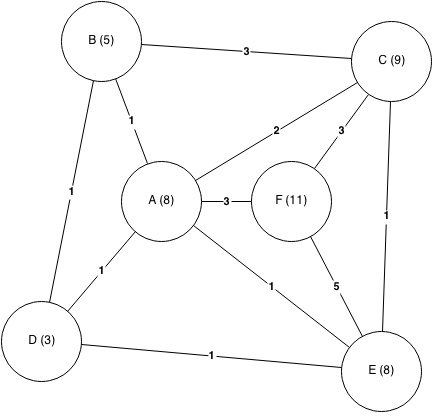
\includegraphics[width=\textwidth]{ejercicio-3-ejemplo-entrada.png}
		\caption{Grafo de entrada}
		\label{fig:ej3_ejemplo}
	\end{minipage}
	\begin{minipage}[t]{0.5\linewidth}
		\centering
		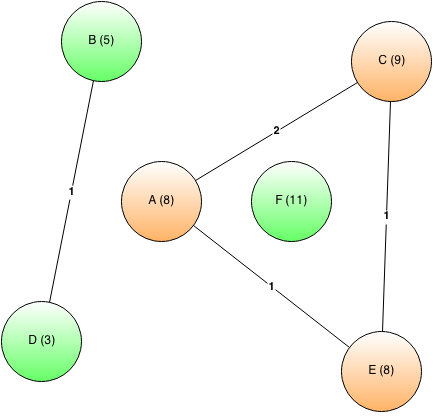
\includegraphics[width=\textwidth]{ejercicio-3-ejemplo-salida.png}
		\caption{La solución dada por la heurística, diferenciada con colores}
		\label{fig:ej3_ejemplo_solucion}
	\end{minipage}
\end{figure}

El problema de la heurística es que solamente compara el peso de un nodo con los conjuntos, sin tener en cuenta el resto de los nodos aún no asignados. Esto puede dar soluciones tan alejadas de la óptima como queramos. A saber:

Sea G un grafo cuyas aristas tienen peso 1, y k el parámetro de k-PMP. Es decir, el grado de un vértice es igual a su peso. G tiene dos tipos diferentes de nodos:
\begin{itemize}
    \item Los nodos $P_1, ..., P_k$ forman un subgrafo completo. Entonces, $d(P_i) = k-1$ en ese subgrafo.
    \item Los nodos $L_1, ..., L_N$ verifican que cada $L_i$ es solamente adyacente a todos los nodos $P_i$. Es decir, $d(L_i) = k$ para todo $i = 1, ..., N$.
\end{itemize}
Por lo anterior, los nodos $P_i$ tienen grado $N+k-1$. Estos nodos van a ser más pesados que los $L_i$ cuando $N > 1$, pues 
\begin{align*}
N+k-1 > k \Longleftrightarrow N > 1
\end{align*}
Supongamos entonces que hay más de un nodo de tipo $L$. Notemos además que el conjunto $\{L_1, ..., L_N\}$ tiene peso cero, ya que ningún par de nodos es adyacente entre sí.
Como el algoritmo ordena por peso de mayor a menor, el orden será del tipo 
\begin{align*}
[P_{i_1},...,P_{i_k},L_{j_1},...,L_{j_N}]
\end{align*}
Entonces, si N $>$ 1, el algoritmo va a elegir un nodo $P$ hasta que se terminen. A $P_{i_1}$ lo va a poner en $S_1$. A $P_{i_2}$ no lo puede poner en $S_1$ porque tiene peso 1 ahí (es adyacente a $P_{i_1}$, por lo tanto lo pone en $S_2$ que está vacío. A $P_{i_3}$ no puede ponerlo ni en $S_1$ ni en $S_2$ por la misma razón, entonces lo pone $S_3$. Así, una vez terminados todos los nodos $P$, la partición es
\begin{align*}
\{\{P_{i_1}\},\{P_{i_2}\},...,\{P_{i_k}\}\}
\end{align*}
Queda insertar los N nodos restantes, que son los $L_{j_1},...,L_{j_N}$. Pero para cualquiera de estos nodos, su peso en $S_x$ es 1 porque es adyacente a $P_{i_x}$. Como el algoritmo elige al primer conjunto y después chequea si eligiendo los demás mejora, y no lo hace en este caso, todos van a ir a $S_1$. Por lo tanto, la solución dada por el algoritmo será
\begin{align*}
\{ \{P_{i_1}, L_1, L_2, ..., L_N\}, \{P_{i_2}\}, ..., \{P_{i_k}\} \}
\end{align*}
El peso total de esta solución es N.
Pero si la solución fuera
\begin{align*}
\{ \{L_1, L_2, ..., L_N\}, \{P_{i_1}, P_{i_2}\}, ..., \{P_{i_k}\} \}
\end{align*}
el peso total sería 1. Es decir, la solución dada por la heurística golosa puede ser tan mala como queramos. Veamos gráficamente para k = 3 la diferencia:
\begin{figure}[H]
	\begin{minipage}[t]{\linewidth}
		\centering
		\frame{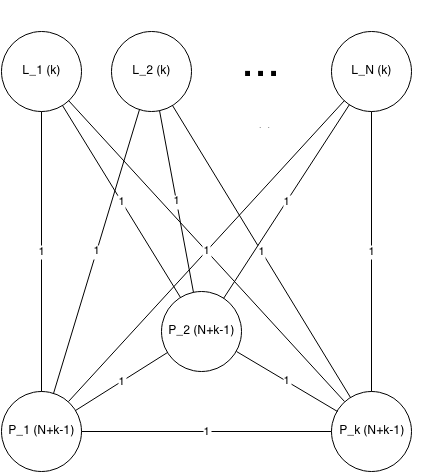
\includegraphics[width=0.5\textwidth]{ejercicio-3-rotura-heuristica.png}}
		\caption{Grafo de entrada}
		\label{fig:ej3_rotura_entrada}
	\end{minipage}
\end{figure}
\begin{figure}[H]
	\begin{minipage}[t]{0.5\linewidth}
		\centering
		\frame{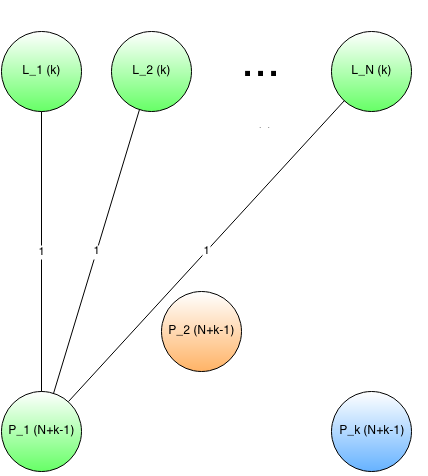
\includegraphics[width=\textwidth]{ejercicio-3-rotura-heuristica-solucion-golosa.png}}
		\caption{Solución golosa, con peso N.}
		\label{fig:ej3_rotura_golosa}
	\end{minipage}
	\begin{minipage}[t]{0.5\linewidth}
		\centering
		\frame{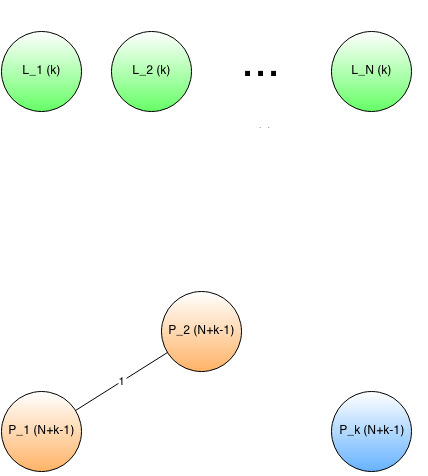
\includegraphics[width=\textwidth]{ejercicio-3-rotura-heuristica-solucion-optima.png}}
		\caption{Una solución óptima, con peso 1.}
		\label{fig:ej3_rotura_optima}
	\end{minipage}
\end{figure}

\subsection{Análisis de complejidad temporal}

Sea $n$ la cantidad de vértices del grafo de entrada, y $k$ el parámetro de k-PMP. Vamos a usar el pseudocódigo ya introducido para el cálculo de complejidad:
\begin{enumerate}
    \item En la primera línea se crean $k$ conjuntos vacíos. Esto cuesta $O(k)$. Llamaremos $C_i$ al i-ésimo conjunto.
    \item Luego, se crea un vector de tamaño $n$, con los vértices ordenados por peso en el grafo, de mayor a menor. Preguntarle a un vértice su peso en el grafo cuesta $O(n)$ porque representamos al grafo con una matriz de adyacencia, entonces en total es $O(n^2)$ saber el peso de todos los nodos. Finalmente, ordenar las tuplas $<nodo,peso(nodo)>$ cuesta $O(n \log n)$. Por lo tanto, todo esto cuesta $O(n^2)$. Al nodo i-ésimo de este nuevo ordenamiento lo llamaremos $u_i$.
    \item Ahora para cada $u_i$ se hace lo siguiente:
        \begin{enumerate}
            \item Inicializar las variables $pesoMinimo$ y $mejorConjunto$ cuesta $O(1)$.
            \item Para cada conjunto $C_i$ de la partición, se calcula el peso de $u_i$ en él y se chequea si es mejor para cambiar el $mejorConjunto$. El peso en un $C_i$ se calcula simplemente sumando los pesos de la aristas adyacentes entre $u_i$ y los vértices del conjunto, lo cual lleva $O(|C_i|)$. Sabemos que
            \begin{align*}
                \sum\limits_{\substack{i = 1}}^k |C_i| &= i - 1
            \end{align*}
            (pues sólo se asignaron $i - 1$ nodos en la iteración i-ésima). Por otro lado, estamos iterando sobre $k$ conjuntos, entonces el costo de este paso es $O(k) + O(i - 1)$.
            \item Insertar el nodo en $mejorConjunto$ cuesta $O(\log |mejorConjunto|)$ que podemos acotar por $O(\log (i - 1))$.
        \end{enumerate}
        En total, todo este paso cuesta
        \begin{align*}
                \sum\limits_{\substack{i = 1}}^n (O(k) + O(i-1) + O(\log (i - 1))) &= O(nk) + O(n^2) + O(\log n!)
        \end{align*}
        Por la aproximación de Stirling del factorial ($\log n! = n \log(n) - n + O(\log n)$), tenemos que $O(\log n!) = O(n \log n)$, entonces la complejidad total de este paso es $O(nk) + O(n^2)$.
\end{enumerate}
Tenemos entonces que la complejidad temporal de la heurística golosa es
\begin{align*}
    T(n,k) &= O(k) + O(n^2) + O(nk) + O(n^2) \\
    T(n,k) &= O(nk) + O(n^2)
\end{align*}
Como tomar valores $k \geq n$ no tiene sentido, ya que una solución óptima es trivial (se toma la partición $\{\{v_1\}, \{v_2\}, ..., \{v_n\}, \{\}, ..., \{\}\}$ que tiene peso total cero), entonces siendo $k < n$ vale que $O(nk) = O(n^2)$. Por lo tanto, la complejidad temporal de peor caso de la heurística para un tamaño de entrada de $n$ vértices es
\begin{align*}
    T(n) &= O(n^2)
\end{align*}

\section{Heurística de búsqueda local}
\subsection{Descripción de los algoritmos}
El procedimiento de una heurística de busqueda local consiste en tomar una solución inicial $s$ cualquiera e iterativamente mejorarla remplazandola por una solución mejor del conjunto de soluciones vecinas ($N(s)$ definidas particularmente en cada algoritmo), hasta llegar a un óptimo local.

Llamamos heurística de busqueda local al método de selección que usamos para elegir o descartar una vecindad. Los algoritmos implementados a continuación usan el mismo criterio de heurística que consiste en iterar sobre las vecindades y elegir la primera que mejora la solución. Usamos este criterio por que mejora el tiempo de ejecución ya que cuando encuentra una mejor la elige y por que no encontramos otra considerablemente mejor. Por ejemplo se podría haber propuesto una heurística que recorra todas las vecindades y elija la mejor opción entre todas, pero aun en el mejor caso deberiamos recorrer todas las soluciones de $N(s)$ y esto incrementa el costo temporal.

Implementamos dos tipos de vecindades: \textbf{(A)} toma un nodo de alguno de los $k$ subconjuntos y prueba si cambiando este nodo de subconjunto mejora el valor de la solución, siendo la vecindad todas las soluciones que difieren de la actual con un solo nodo en otro subconjunto $k$. \textbf{(B)} consiste en intercambiar dos nodos cualesquiera de distintos subconjuntos y ver si el valor mejora, es decir que la vecindad son aquellas soluciones que difieren solamente con un intercambio de nodos en dos distintos subconjuntos.

Consideramos que la implementación que tiene la vecindad de tipo \textbf{(B)} es más limitada que la \textbf{(A)} porque la \textbf{(B)} mantiene la cardinalidad en los subconjuntos de la solución (ya que solo hace swap entre nodos de distintos subconjuntos) y esto hace que el algoritmo este más condicionado por la solución de partida.

\textbf{(A)}:
\begin{algorithm}[H]
\begin{algorithmic}[1]
\caption{HeuristicaBusquedaLocal(Grafo G, nat k)}
\STATE Vector$<$Conjunto$<$Nat$>>$ conjuntos(k, vacío)
\STATE solucionInicial(G,k)
\STATE Bool hayMejora $\leftarrow$ true
\WHILE {hayMejora}
    \STATE hayMejora $\leftarrow$ false
    \FOR {\textbf{each} nodos}
        \STATE Bool swappeado $\leftarrow$ false
        \STATE Int subset $\leftarrow$ 0
        \WHILE {!swappeado y subset $<$ k}
            \IF{subset != subcjtoDel(nodo) y pesoDelNodoEnSubcjto(actual) $>$ pesoDelNodoEnSubcjto(subset)}
                \STATE borroNodoDeSubcjto(nodo,actual)
                \STATE agregoNodoASubcjto(nodo,subset)
                \STATE hayMejora $\leftarrow$ true
                \STATE swappeado $\leftarrow$ true
            \ENDIF
            \STATE subset++
        \ENDWHILE
    \ENDFOR
\ENDWHILE
\RETURN conjuntos
\end{algorithmic}
\end{algorithm}

\textbf{(B)}:
\begin{algorithm}[H]
\begin{algorithmic}[1]
\caption{HeuristicaBusquedaLocalConSwap(Grafo G, nat k)}
\STATE Vector$<$Conjunto$<$Nat$>>$ conjuntos(k, vacío)
\STATE solucionInicial(G,k)
\STATE Bool hayMejora $\leftarrow$ true
\WHILE {hayMejora}
    \STATE hayMejora $\leftarrow$ false
    \FOR {\textbf{each} nodos}
        \STATE Bool swappeado $\leftarrow$ false
        \STATE nodoSwap $\leftarrow$ nodo$+1$
        \WHILE {!swappeado y nodoSwap $<$ n}
            \IF{subcjtoDel(nodo) != subcjtoDel(nodoSwap)}
                \STATE pesoNodoCambiado $\leftarrow$ pesoDelNodoEnSubcjto(nodo,subcjtoDel(nodoSwap))
                \STATE pesoNodoSwapCambiado $\leftarrow$ pesoDelNodoEnSubcjto(nodoSwap,subcjtoDel(nodo))
                \IF{peso(nodo)$+$peso(nodoSwap) $>$ pesoNodoCambiado$+$pesoNodoSwapCambiado}
                    \STATE borroNodoDeSubcjto(nodo,subcjtoDel(nodo))
                    \STATE agregoNodoASubcjto(nodo,subcjtoDel(nodoSwap))
                    \STATE borroNodoDeSubcjto(nodoSwap,subcjtoDel(nodoSwap))
                    \STATE agregoNodoASubcjto(nodoSwap,subcjtoDel(nodo))
                    \STATE hayMejora $\leftarrow$ true
                    \STATE swappeado $\leftarrow$ true
                \ENDIF
            \ENDIF
            \STATE nodoSwap++
        \ENDWHILE
    \ENDFOR
\ENDWHILE
\RETURN conjuntos
\end{algorithmic}
\end{algorithm}

Ejemplo de ejecución de los algoritmos:

Tenemos el siguiente grafo de entrada, y nos piden correr los algoritmos para $k=3$

\begin{figure}[H]
    \centering
    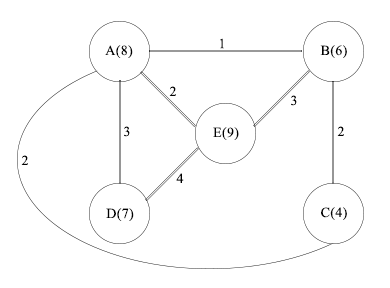
\includegraphics[scale=0.7]{ejercicio-4-ejemplo-entrada.png}
    \caption{Grafo de entrada}
    \label{fig:ej4_ejemplo}
\end{figure}

Contamos con la siguiente solución inicial (entre parentesis el peso de cada nodo):
\begin{center}
  \begin{tabular}{ l | c | r }
    $S_{1}$ & $S_{2}$ & $S_{3}$ \\ \hline
    A(3) & E(0) & D(0) \\
    B(4) &  &  \\
    C(3) &  &  \\
  \end{tabular}
  \textbf{Costo total:} 5
\end{center}

\begin{minipage}[t]{0.5\linewidth}
    \center{\textbf{(A)}} \\
    \raggedright{
        \textit{Tomo A:}\\
        $\rightarrow$ Lo pruebo en $S_{2}$: A(2) \checkmark Mejora
    }\\
    \begin{center}
      \begin{tabular}{ l | c | r }
        $S_{1}$ & $S_{2}$ & $S_{3}$ \\ \hline
        B(2) & E(2) & D(0) \\
        C(2) & A(2) &  \\
      \end{tabular}
      \textbf{Costo total:} 4
    \end{center}

    \raggedright{
        \textit{Tomo B:}\\
        $\rightarrow$ Lo pruebo en $S_{2}$: B(4) No mejora\\
        $\rightarrow$ Lo pruebo en $S_{3}$: B(0) \checkmark Mejora
    }\\
    \begin{center}
      \begin{tabular}{ l | c | r }
        $S_{1}$ & $S_{2}$ & $S_{3}$ \\ \hline
        C(0) & E(2) & D(0) \\
         & A(2) & B(0) \\
      \end{tabular}
      \textbf{Costo total:} 2
    \end{center}

    \raggedright{
        \textit{Tomo C:}\\
        $\rightarrow$ Lo pruebo en todos pero no mejora en ninguno por que tiene peso 0.
    }\\

    \raggedright{
        \textit{Tomo D:}\\
        $\rightarrow$ Lo pruebo en todos pero no mejora en ninguno por que tiene peso 0.
    }\\

    \raggedright{
        \textit{Tomo E:}\\
        $\rightarrow$ Lo pruebo en $S_{1}$: E(0) \checkmark Mejora
    }\\
    \begin{center}
      \begin{tabular}{ l | c | r }
        $S_{1}$ & $S_{2}$ & $S_{3}$ \\ \hline
        C(0) & A(0) & D(0) \\
        E(0) &  & B(0) \\
      \end{tabular}
      \textbf{Costo total:} 0
    \end{center}

    Hace una iteración mas buscando mejora pero no la encuentra, entonces termina. 

\end{minipage}
\vrule
\begin{minipage}[t]{0.5\linewidth}
    \centering{\textbf{(B)}}\\
    \raggedright{
        \textit{Tomo A y B:}\\
        $\rightarrow$ estan en el mismo subconjunto (no hago nada).
    }\\
    \raggedright{
        \textit{Tomo A y C:}\\
        $\rightarrow$ estan en el mismo subconjunto.
    }\\
    \raggedright{
        \textit{Tomo A y D:}\\
        $\rightarrow$ como peso(A en $S_{3}$ sin D)$+$peso(D en $S_{1}$ sin A) $<$ peso(A actual)+peso(D actual)
    }\\
    \begin{center}
      \begin{tabular}{ l | c | r }
        $S_{1}$ & $S_{2}$ & $S_{3}$ \\ \hline
        B(2) & E(0) & A(0) \\
        C(2) &  &  \\
        D(0) &  &  \\
      \end{tabular}
      \textbf{Costo total:} 2
    \end{center}
    \raggedright{
        \textit{Tomo B y A:}\\
        $\rightarrow$ no mejora.
    }\\
    \raggedright{
        \textit{Tomo B y C:}\\
        $\rightarrow$ estan en el mismo subconjunto.
    }\\
    \raggedright{
        \textit{Tomo B y D:}\\
        $\rightarrow$ estan en el mismo subconjunto.
    }\\
    \raggedright{
        \textit{Tomo B y E:}\\
        $\rightarrow$ no mejora.
    }\\
    \raggedright{
        \textit{Tomo C y A:}\\
        $\rightarrow$ no mejora.
    }\\
    \raggedright{
        \textit{Tomo C y B:}\\
        $\rightarrow$ estan en el mismo subconjunto.
    }\\
    \raggedright{
        \textit{Tomo C y D:}\\
        $\rightarrow$ estan en el mismo subconjunto.
    }\\
    \centering{...}\\
    No mejora en ninguna de las combinaciones siguientes.
    Termina.


\end{minipage}


\subsection{Análisis de complejidad temporal}
Sea $n$ la cantidad de vértices del grafo de entrada, y $k$ el parámetro de k-PMP. Vamos a usar el pseudocódigo ya introducido para el cálculo de complejidad de ambos algoritmos. Hay que mencionar que ésta se calcula para el peor caso de una iteración del ciclo más exterior de los algoritmos (\textit{while(hayMejora)}) ya que no podemos determinar cuantas veces se itera sobre este mismo. Lo que si se afirma es que termina cuando encuentra un óptimo local, es decir ninguno de sus vecinos tiene una mejor solución. Se omite la complejidad de la obtención de la solución inicial y se asume como entrada.
\\

\textbf{(A):}

\begin{itemize}
    \item Linea $5$: seteamos la variable \textit{hayMejora} en $O(1)$
    \item Linea $6$: iniciamos un ciclo que se repite n veces.
    \begin{itemize}
        \item Lineas $7$ y $8$: seteamos variables en $O(1)$ y calculamos el peso del nodo en cuestión en el subconjunto esto cuesta $O(n)$ (si bien no está explícito en el pseudocódigo, realizamos este preproceso para no realizarlo dentro del ciclo siguiente y así aumentar su complejidad innecesariamente.)
        \item Linea $9$: Se inicia otro ciclo sobre los subconjuntos que como peor caso se prueba cambiar el nodo a todos los subconjuntos y recorremos los $k$.
        \begin{itemize}
            \item Linea $10$: Checkeo booleano del if en $O(1)$
            \item Lineas $11$, $12$, $13$ y $14$: borrar e insertar nodos de un conjunto cuesta $O(\log n)$ y las asignaciones de variables $O(1)$. 

            Entonces tenemos $2O(\log n) + 2O(1)$

            Cómo peor caso esto ocurre una vez en las $k$ iteraciones ya que hace que salgamos de él.
            \item Linea $16$: aumentamos una variable en $O(1)$
        \end{itemize}
    \end{itemize}
\end{itemize}
Entonces tenemos:
\begin{center}
    $Complejidad(A) = O(1) + n(O(1)+O(n)+O(k)+2O(\log n)+2O(1)+O(1))$

    $Complejidad(A) = n(max\{O(n),O(k),O(\log n)\})$

    $Complejidad(A) = max\{O(n^2),O(nk),O(n\log n)\}$

    $Complejidad(A) = O(n^2)$
\end{center}

\textbf{(B):}

\begin{itemize}
    \item Linea $5$: seteamos la variable \textit{hayMejora} en $O(1)$
    \item Linea $6$: iniciamos un ciclo que se repite n veces.
    \begin{itemize}
        \item Lineas $7$ y $8$: seteamos variables en $O(1)$ y calculamos los pesos de ambos nodos en los dos subconjuntos, esto cuesta $4O(n)$ (esto lo hacemos para no calcularlos dentro del siguiente ciclo.)
        \item Linea $9$: Se inicia otro ciclo sobre los nodos (para checkear con quien swappeo) en peor caso se repita $n$ veces.
        \begin{itemize}
            \item Linea $10$: Checkea booleano del if en $O(1)$
            \item Lineas $11$ y $12$: Calcula el valor del peso del nodo en un subconjunto, como peor caso esto toma $O(n)$
            \item Linea $13$: Checkea booleano del if en $O(1)$
            \item Lineas $14$ a $19$: Borra e inserta nodos de un subconjunto a otro, cuesta $O(\log n)$ y las asignaciones de variables $O(1)$. 

            Entonces tenemos $4O(\log n) + 2O(1)$

            Cómo peor caso esto ocurre una vez en las $n$ iteraciones ya que hace que salgamos de él.
            \item Linea $16$: aumentamos una variable en $O(1)$
        \end{itemize}
    \end{itemize}
\end{itemize}

Entonces tenemos:
\begin{center}
  $Complejidad(B) = O(1) + n(O(1)+4O(n)+n(O(n)+4O(\log n)+2O(1))+O(1))$

  $Complejidad(B) = n(O(n)+O(n^2))$ 

  $Complejidad(B) = O(n^3)$
\end{center}

\subsection{Experimentación de calidad}
Con esta experimentación nos interesan ver dos cosas:

\begin{enumerate}
  \item cuál de las dos vecindades obtiene soluciones de mejor calidad.
  \item cuál de las dos vecindades \textit{gana} más veces que la otra. 
    Por ganar nos referimos a que obtiene una partición de menor peso.
\end{enumerate}

Para evaluarlo generamos un set de instancias que se compone de 100 instancias por $n$, siendo
$n$ la cantidad de nodos de la instancia, con $3 \leq n \leq 22$. La limitante para aumentar más
el $n$ es que el tiempo del exacto, incluso con todas las podas, crece demasiado rápido y para
poder saber cuán lejos estaban los pesos obtenidos por las heurísticas de búsqueda local era necesario
correr el algoritmo exacto. En todas las instancias las búsquedas para las dos vecindades parten de
la misma partición inicial que es la generada por el goloso sin aleatorización. Creemos que 
empezar desde la solución obtenida por la golosa se acerca un más al uso real que va a tener en 
comparación con empezar con una partición completamente aleatoria, por lo cual los resultados que
obtengamos serán más representativos del comportamiento que vayan a tener en su contexto de uso.
Los valores graficados se corresponden con los promedios de pesos por instancia. Es necesario
aclarar que limitamos el número de iteraciones de las dos búsquedas locales a 100. Creemos
que esto es importante ya que no sólo nos interesa controlar que la calidad de las soluciones que 
estamos comparando hayan sido obtenidas dentro de el mismo número de iteraciones. De no haber hecho esto
una de las dos podría haber superado a la otra pero realizando muchas más iteraciones. Sumamos los pesos
obtenidos para las 100 instancias de cada $n$ y luego tomamos el promedio. El promedio no es un buen 
indicador en muchos casos ya que no nos habla en general de la dispersión de los resultados. Para
darnos una idea de cuán estable son los resultados que obtienen cada una de las vecindades necesitaríamos
obtener también el desvío estándar. Sin embargo, los promedios de las dos vecindades han quedado con error
relativo pequeño con respecto al peso obtenido por el algoritmo exacto por lo cual el desvío estándar debe ser pequeño
ya que no pueden haber valores por debajo del exacto para compensar otros muy altos.

\begin{figure}[H]
		\centering
		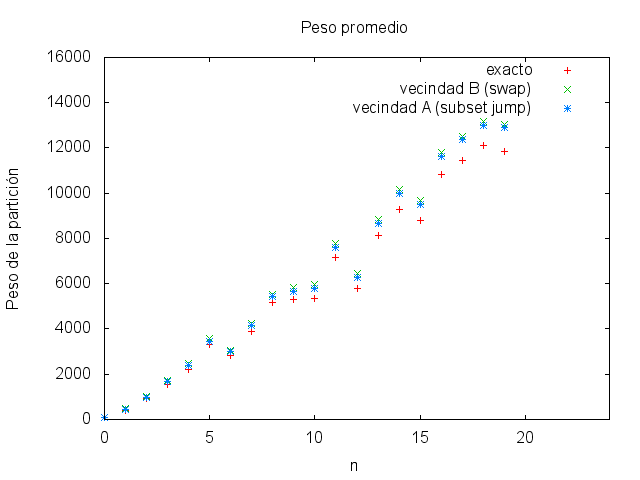
\includegraphics[width=\textwidth]{calidad_trendline.png}
		\caption{Pesos promedio.}
		\label{fig:ej3_ejemplo}
\end{figure}

La distancia entre los pesos obtenidos por las vecindades y el exacto se mantiene parece estar creciendo.
No obstante, la distancia entre las dos vecindades se mantiene, a simple vista, constante. La vecindad A, que
corresponde a la que cambia de subconjunto a un nodo, siempre se ubica por debajo de la vecindad B, correspondiente
a la de swap, pero por un margen muy pequeño. Sobre todo para las instancias donde el $n$ es más grande, superior
a 15, los resultados dejan de seguir una curva suave lo cual interpretamos que se debe a que 100 instancias a medida
que el $n$ aumenta deja de ser un valor representativo.
Además, realizamos un histograma que muestra para cada $n$ qué vecindad obtuvo el menor peso de las dos para cada una
de las 100 instancias. De esta forma podemos ver más claramente cuál ganó más veces, otro indicador de cuál podría
llegar a ser superior.

\begin{figure}[H]
		\centering
		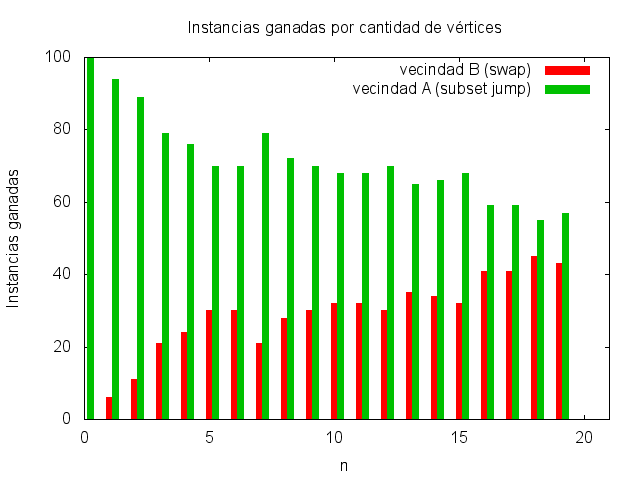
\includegraphics[width=\textwidth]{calidad_histograma.png}
		\caption{Instancias ganadas.}
		\label{fig:ej3_ejemplo}
\end{figure}

Vemos que la vecindad A comienza con una ampli ventaja sobre la vecindad B pero a medida que el $n$ aumenta
se va emparejando cada vez más. Ésta es una tendendia que no habíamos podido apreciar en el gráfico de pesos.
No estamos seguros si se debe a como ya mencionamos la falta de representatividad de las 100 instancias para
los $n$ más grandes o a que efectivamente la vecindad A obtiene soluciones de mejor calidad en la mayoría de los
casos.

\subsection{Experimentación de complejidad}
En esta experimentación simplemente queremos ganar confianza en las cotas de complejidad
calculadas teóricamente. Recordamos que para la vecindad A (cambio de subconjunto) la cota obtenida
había sido $O(n^2)$. Lo que hicimos fue correr el mismo conjunto de instancias que para la experimentación
de calidad pero aumentando el rango de valores de que toma $n$ ya que en este caso no es necesario correr
el algoritmo exacto que nos limitaba anteriormente. Los tiempos están divididos por $n$.

\begin{figure}[H]
		\centering
		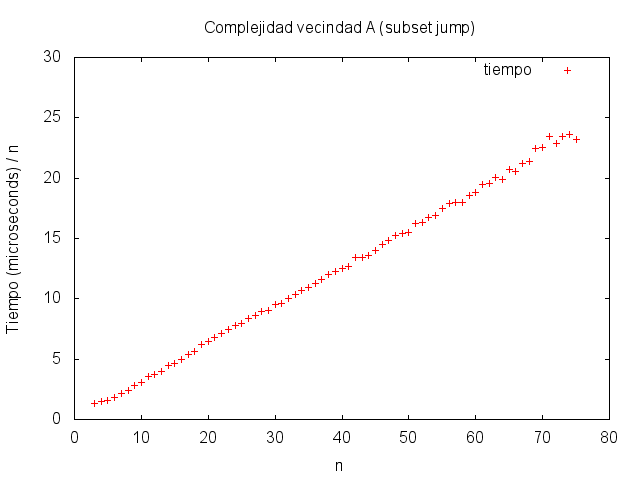
\includegraphics[width=\textwidth]{tiempos_vecindad_a.png}
		\caption{Instancias ganadas.}
		\label{fig:ej3_ejemplo}
\end{figure}

Los tiempos parecen presentar un comportamiento bastante definido incluso para valores de $n$ más grandes
por lo cual creemos que la cota de complejidad se acerca lo suficiente a la real.
Realizamos lo mismo para la vecindad B (swap). Recordamos que la cota obtenida para ésta vecindad era $O(n^3)$
por lo cual dividimos los tiempos por $n^2$.

\begin{figure}[H]
		\centering
		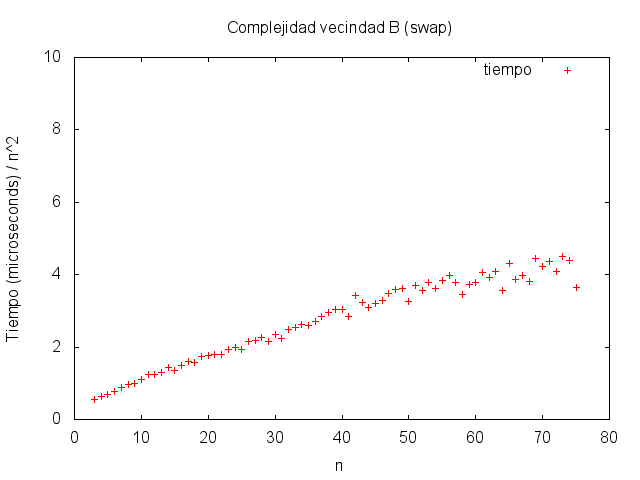
\includegraphics[width=\textwidth]{tiempos_vecindad_b.png}
		\caption{Instancias ganadas.}
		\label{fig:ej3_ejemplo}
\end{figure}

En este caso vemos que si bien parece que los valores exhiben un crecimiento lineal, a partir de $n = 40$
esta tendencia se vuelve cada vez más endeble ya que los valores empiezan a presentar turbulencia. Creemos
que una vez más esto puede deberse a la falta de representatividad de un valor de sólo 100 instancias para
un número de nodos tan grandes, lo cual podría resultar en instancias muy densas y otras muy simples.
Concluimos que la vecindad A por tener una complejidad menor y mostrarse levemente superior en cuanto
a calidad de las soluciones obtenidas con respecto a la vecindad B será una mejor elección para nuestra
implementación de la metaheurística GRASP.

\section{Ejercicio 5}

\subsection{Tests}
Mostraremos los resultados de varios tests realizados a la GRASP, que introducimos brevemente a continuación:
\begin{itemize}
    \item \textbf{Test de configuración}: Dado un conjunto de instancias, busca la mejor configuración de la GRASP, variando criterios de parada y de selección de la lista de candidatos (RCL) de la heurística golosa aleatorizada.
    \item \textbf{Test de calidad}: Para un conjunto reducido de instancias, se compara cuánto más pesada es la solución de la GRASP en relación a la solución óptima, usando la configuración ganadora del test anterior.
    \item \textbf{Test de tiempo de ejecución}: Dado un conjunto de instancias, se calculan los tiempos de ejecución de la GRASP para distintas configuraciones.
\end{itemize}

El conjunto de instancias utilizado está compuesto por 100 instancias para cada \\ ${n = 3, ..., 100}$ y tiene las siguientes características:
\begin{enumerate}
    \item Los pesos de las aristas de los grafos pertenecen al intervalo cerrado $[\num{0.0001}, \num{1000}]$.
    \item Sea $G = (V,X)$ con $n = |V|$ y $m = |X|$ un grafo cualquiera del conjunto.\\ Sea $m_{max} = \frac{n(n-1)}{2}$. Entonces,
            \begin{align*}
                \num{0.7} \cdot m_{max} \leq m \leq m_{max} 
            \end{align*}
            Esto lo hicimos para evitar tener instancias con grafos fáciles de resolver incluso para la heurística golosa. Esto es claro en el caso extremo de que el grafo no tenga aristas. Teniendo esto en cuenta, pedimos que al menos tengan $70\%$ de la máxima cantidad de aristas posibles para cada grafo.
    \item Sea $G = (V,X)$ con $n = |V|$ un grafo cualquiera del conjunto. Entonces,
            \begin{align*}
                        2 \leq k \leq max\left(2, \frac{n}{3}\right)
            \end{align*}
            La razón de esto es la misma que en el punto anterior. En el caso extremo, si tuviéramos un grafo con $k \geq n$, alcanzaría con poner un vértice en cada conjunto para obtener una solución óptima (en el otro extremo, $k = 1$ sólo admite una solución, que obviamente es óptima). A mayor $k$, más márgen de error se le da a la heurística para equivocarse porque tiene más conjuntos donde colocar vértices. Por este motivo limitamos a $\frac{n}{3}$ la cantidad de conjuntos que puede tener una partición.
\end{enumerate}
Las instancias fueron generadas aleatorizando cada una de las variables mencionadas. El código del generador se encuentra en el Apéndice.


\subsubsection{Test de configuración}

Lo que primero necesitamos es tener una idea de cuál configuración usar en la GRASP. Para ello, testearemos con todas las combinaciones de configuraciones para un set acotado de valores, y discutiremos al respecto sobre cómo interpretar los resultados obtenidos, y así decidir una configuración.

Tenemos dos criterios de parada: parar por un límite $\alpha$ de iteraciones máximo, o parar si una cierta cantidad $\beta$ de instancias pasaron sin haber mejora en la solución. Por el el lado de la heurística aleatorizada, es decir, para la selección de candidatos, tenemos dos variables independientes: la profundidad de la elección del próximo vértice a insertar, y la profundidad de la elección del conjunto en que va a ser insertado el vértice.

Parar por un máximo de iteraciones $\alpha$ es el criterio más sencillo, pero tiene inconvenientes. Por un lado, podemos estar haciendo muchas iteraciones de más ya que rápidamente encontramos la solución óptima; esto ocurre siempre con grafos con pocos nodos, que son fáciles de resolver. Por otro lado, puede pasar que la cantidad fija de iteraciones que fue seteada no sea suficiente, y que obtengamos soluciones subóptimas incluso para lo que puede dar GRASP.

Parar por iteraciones sin mejora es más flexible porque si se encuentra rápidamente la solución óptima, no va a haber mejora en las próximas $\beta$ iteraciones, por lo cual el algoritmo va a terminar mucho más rápido para este tipo de casos. Para el caso en que sí haya mejoras todo el tiempo, incluso aunque $\beta < \alpha$ el algoritmo seguirá ejecutando hasta que pasen $\beta$ iteraciones sin mejorar, lo cual puede hacer que el total de iteraciones sea mucho mayor a $\alpha$, pero consiguiendo una solución con mejor calidad que parar por máximo de iteraciones. De todas formas, podría pasar que las soluciones obtenidas de la golosa y mejoradas con la búsqueda local, sean peores que la mejor hasta el momento durante $\beta$ iteraciones, y que si $\beta < \alpha$, se termine haciendo menos iteraciones que $\alpha$, por lo cual no hay garantía de que parar por iteraciones sin mejora en el caso $\beta < \alpha$ vaya a devolver mejores soluciones que parar en $\alpha$ iteraciones.

Si tomamos $\beta < \alpha$, cabe preguntarse qué valor de $\beta$ hace falta para que parar por iteraciones sin mejora sea mejor que parar por máximo de iteraciones. Fijamos $\alpha = 100$, y testeamos con $\beta = 10, 35, 50, 70$.

Pero todavía falta la selección de candidatos: plantearemos que ambas profundidades puedan tomar los valores $1$, $2$ ó $4$. Como notación, cuando decimos \underline{profundidad $(x_1,x_2)$} significa profundidad de elección de vértice $x_1$ y profundidad de elección de conjunto $x_2$. Notar que la profundidad $(1,1)$ es equivalente a la golosa pura, sin aleatoriedad. Dejamos esa opción para verificar que la aleatoriedad es efectivamente necesaria para obtener mejores soluciones. Con respecto a esto, conjeturamos que lo mejor es aleatorizar lo máximo posible, entonces esperamos ver que $(4,4)$ sea la mejor configuración de selección.

Dado un $n$, para cada instancia que tenga un grafo de $n$ nodos, se va ejecutar GRASP con cada configuración por separado y se van a acumular los resultados. Luego, se busca cuál es la mejor configuración para este $n$ hallando el mínimo de las sumas de pesos para cada configuración. El mínimo se calcula de la siguiente manera:
\begin{algorithm}[H]
\begin{algorithmic}[1]
\caption{Cálculo del mínimo peso de las configuraciones para un $n$}
\STATE mejorPesoAcumulado $\leftarrow$ $+ \infty$
\FOR {valor de iteraciones sin mejora (10, 35, 50, 70)}
    \FOR{cada valor de profundidad de vértice (4, 2, 1)}
        \FOR{cada valor de profundidad de conjunto (4, 2, 1)}
            \IF{Peso acumulado de esta configuración $<$ mejorPesoAcumulado}
                \STATE Actualizar mejorPesoAcumulado
                \STATE Poner la actual como mejor configuración
            \ENDIF
        \ENDFOR
    \ENDFOR
\ENDFOR
\FOR {valor de máximo de iteraciones (100)}
    \FOR{cada valor de profundidad de vértice (4, 2, 1)}
        \FOR{cada valor de profundidad de conjunto (4, 2, 1)}
            \IF{Peso acumulado de esta configuración $<$ mejorPesoAcumulado}
                \STATE Actualizar mejorPesoAcumulado
                \STATE Poner la actual como mejor configuración
            \ENDIF
        \ENDFOR
    \ENDFOR
\ENDFOR
\end{algorithmic}
\end{algorithm}
Empezamos buscando el mínimo parando por iteraciones sin mejora, y después de encontrarlo, vemos si por máximo de iteraciones es mejor para ese $n$. Dentro de cada configuración de parada, calculamos para cada profundidad (recorriéndolas de esta manera: $(4,4)$, $(4,2)$, $(4,1)$, $(2,4)$, etc). Si como conjeturamos, $(4,4)$ es la mejor profundidad, las demás no deberían dar pesos acumulados menores, y debería ganar siempre $(4,4)$. Lo mismo para el criterio de parada, si parar por 10 iteraciones consigue la solución óptima, y las demás configuraciones no la mejoran, ésa es la elegimos como mejor porque hizo menos iteraciones que las demás.

Por otro lado, para el total del conjunto de instancias hacemos esta misma acumulación de pesos también separando por configuración, y buscamos de esta manera obtenemos la configuración de mínimo peso en las 10.000 instancias.

Veamos primero cuál de los dos criterios de parada resultó ganador para cada $n$. El siguiente gráfico se interpreta de la siguiente manera: Si y(n) es 10, 35, 50, ó 70, entonces ganó iteraciones sin mejora con valor y(n). Si es 100, entonces ganó máximo de iteraciones, con ese valor (que es el único).
\begin{figure}[H]
    \begin{minipage}[t]{\linewidth}
		\centering
		\frame{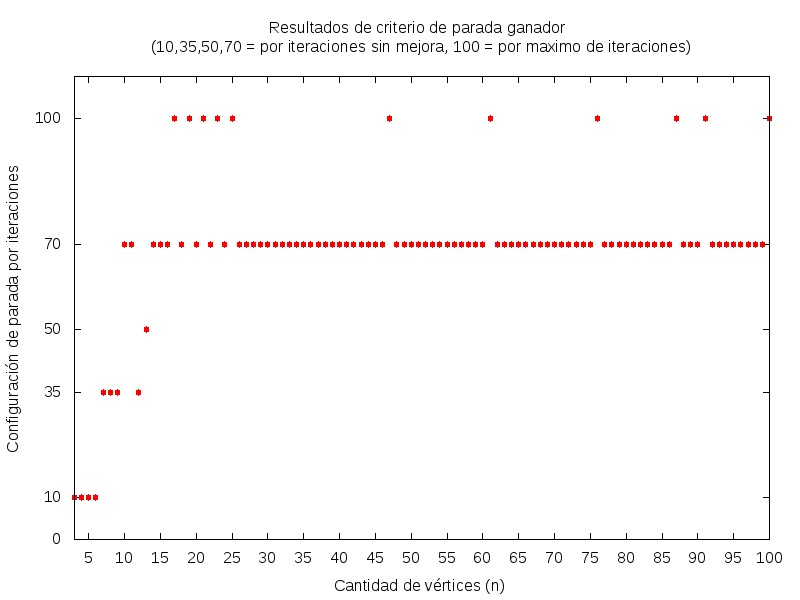
\includegraphics[width=\textwidth]{ejercicio-5-configuracion-conjunto-1.jpg}}
		\label{fig:ejercicio-5-configuracion-conjunto-1}
    \end{minipage}
\end{figure}
Podemos observar que para valores de $n$ menores a 15, muchas veces alcanza con 10, 35 ó 50 iteraciones sin mejora para ganar; es decir, en ningún caso usar las 100 iteraciones del otro criterio de parada mejora la solución, como preveíamos. Pero al aumentar el $n$, aunque claramente parar por 70 iteraciones sin mejora gana más veces, observamos que a veces resulta mejor el criterio de máximo de iteraciones, lo cual muestra falta de garantía de parar por iteraciones sin mejora.

Independientemente de qué criterio de parada sea mejor para cada $n$, veamos qué profundidad resultó ganadora. Veamos primero para cuantos $n$ resultó ganadora cada una:
\begin{figure}[H]
    \begin{minipage}[t]{\linewidth}
		\centering
		\frame{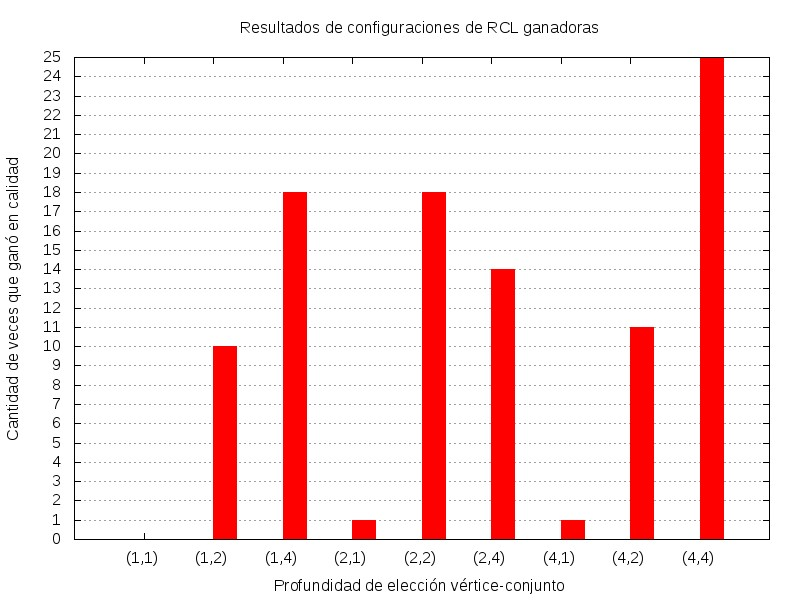
\includegraphics[width=\textwidth]{ejercicio-5-histograma-rcl-conjunto-1.jpg}}
		\label{fig:ejercicio-5-histograma-rcl-conjunto-1}
    \end{minipage}
\end{figure}
La primera observación es que usar de profundidad $(x,1)$ no es conveniente. En particular, $(1,1)$, que es equivalente a que la heurística golosa no tenga aleatoriedad, no resultó ganadora para ningún caso, como esperábamos. Usar $(4,4)$ gana más veces (25), y usar $(x,4)$ gana 57 veces, contra 39 ganadas de $(x,2)$. Fijando los conjuntos, $(1,x)$ gana 28 veces, $(2,x)$ gana 33, y $(4,x)$ gana 37 veces. Hasta ahora pareciera que $(4,4)$ es la mejor profundidad, pero tenemos que ver más detalladamente qué ocurre para cada $n$, porque si por ejemplo $(4,4)$ sólo ganara para las primeros 25 cantidades de nodos, pero fuera superada para $n \geq 27$, claramente sería una profundidad que no funciona para grafos con una cantidad elevada de nodos. Veamos entonces cuál profundidad gana para cada $n$:
\begin{figure}[H]
    \begin{minipage}[t]{\linewidth}
		\centering
		\frame{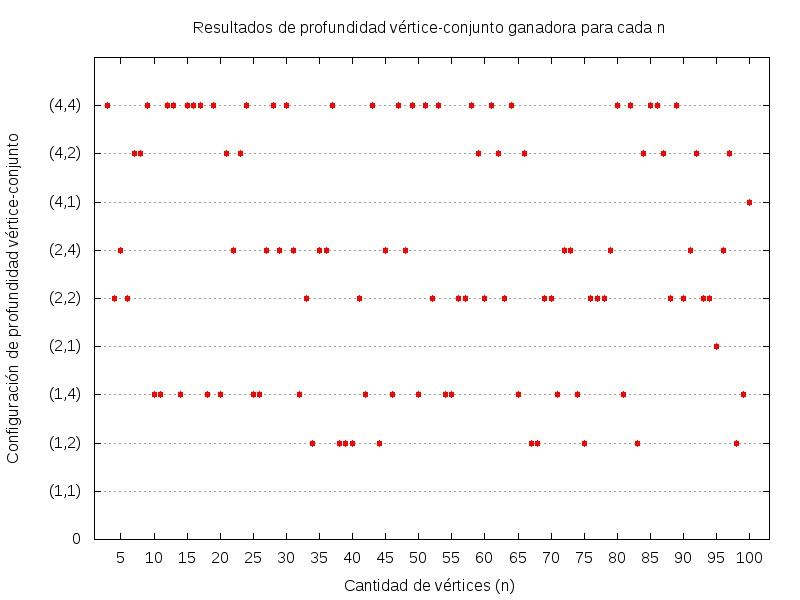
\includegraphics[width=\textwidth]{ejercicio-5-configuracion-profundidad-conjunto-1.jpg}}
		\label{fig:ejercicio-5-configuracion-profundidad-conjunto-1}
    \end{minipage}
\end{figure}
Podemos ver en el gráfico que $(4,4)$ gana de manera consistente, excepto para los $n$ más altos, para los cuales no parece haber claramente un ganador, ya que ganan casi todas las configuraciones. Hay un problema más: no sabemos exactamente por cuánto gana una profundidad. Vamos a usar el cálculo paralelo que hicimos, la suma de los pesos de cada configuración para las 10.000 instancias, para ver qué tan alejadas están verdaderamente las configuraciones de profundidad. Veamos los pesos acumulados de iteraciones sin mejora con valor 70 para cada profundidad $(x,y)$:
\begin{table}[H]
    \begin{center}
        \begin{tabular}{ | l | l | l | l |}
        \hline
        (x,y)   & 1                 & 2                 & 4 \\ \hline
        1       & 459037888         & 432225472         & 432218464 \\ \hline
        2       & 433368064         & 432117408         & 432198464 \\ \hline
        4       & 432523232         & 432218784         & 432113312 \\
        \hline
        \end{tabular}
        \caption{Peso acumulado para cada configuración}
    \end{center}
\end{table}
\begin{table}[H]
    \begin{center}
        \begin{tabular}{ | l | l | l | l |}
        \hline
        (x,y)   & 1                 & 2                 & 4 \\ \hline
        1       & 6.2309\%         & 0.0259\%         & 0.0243\% \\ \hline
        2       & 0.2903\%         & 0.0009\%         & 0.0197\% \\ \hline
        4       & 0.0948\%         & 0.0244\%         & 0.0000\% \\
        \hline
        \end{tabular}
        \caption{Error relativo de cada configuración contra el peso de la configuración $(4,4)$}
    \end{center}
\end{table}
$(4,4)$ logra el menor peso, y $(1,1)$ el peor (siendo $6.23\%$ más pesada). En particular, la primera columna, es decir, las profundidades $(x,1)$ son las tres peores. Pero el resto de las configuraciones no son mucho más pesadas que $(4,4)$ (la más pesada de éstas, $(1,2)$, sólo es un $0.026\%$ más pesada. En particular, $(2,2)$ es la más cercana siendo sólamente $0.0009479\%$ más pesada. Si tuviéramos que elegir entre fijar alguna profundidad en 1, y poder variar la otra, claramente podemos sacar como conclusión que aleatorizar la elección del conjunto es más importante que aleatorizar la elección del vértice a insertar. Aunque por otro lado, vemos que aumentar la profundidad de la elección de vértices también mejora las soluciones.

\noindent Por todo lo anterior, decidimos usar la configuración siguiente:
\begin{itemize}
    \item Criterio de parada: iteraciones sin mejora.
    \item Profundidad elección vértice-conjunto: $(4,4)$.
\end{itemize}

\subsubsection{Test de calidad}

En este test comparamos los pesos de las soluciones dadas por la GRASP con la configuración que elegimos (iteraciones sin mejora y profundidad $(4,4)$), contra los pesos de las soluciones óptimas obtenidas del algoritmo exacto. Lo hicimos hasta $n = 23$ por la complejidad temporal no polinomial del algoritmo exacto. 

Variamos el límite de iteraciones en potencias de 2: tomamos los valores $2^i$ con $i = \{0,1,...,9\}$. Para cada uno, calculamos el promedio de los errores relativos (en porcentaje) de las intancias de $n$ nodos, para $n = \{3,4,...,23\}$. Veamos los resultados:

\begin{figure}[H]
    \begin{minipage}[t]{\linewidth}
		\centering
		\frame{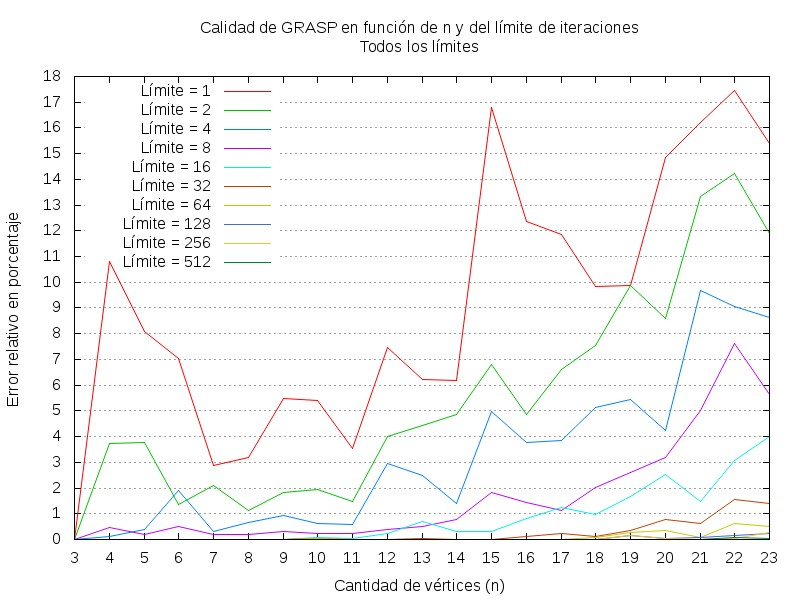
\includegraphics[width=\textwidth]{ejercicio-5-calidad-todos-conjunto-1.jpg}}
		\label{fig:ejercicio-5-calidad-todos-conjunto-1}
    \end{minipage}
\end{figure}

Como era de esperar, a mayor límite de iteraciones, mejor solución devuelve la GRASP. Tomar como límite una sola iteración tiene la peor performance, superando en el peor caso el $17\%$. Además, podemos ver que el error relativo para cualquier valor de iteraciones aumenta con el $n$, lo cual sugiere que no alcanza con fijar un cierto límite si no se sabe la máxima cantidad de vértices que van a tener los grafos de las instancias de entrada.

Veamos más en detalle lo que ocurre con los límites de iteraciones más altos, que dan los mejores resultados:

\begin{figure}[H]
    \begin{minipage}[t]{\linewidth}
		\centering
		\frame{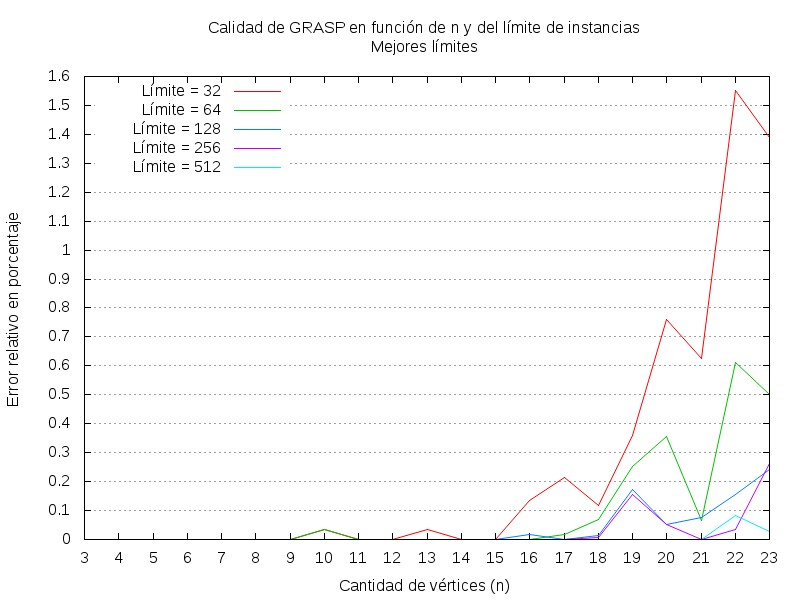
\includegraphics[width=\textwidth]{ejercicio-5-calidad-mejores-conjunto-1.jpg}}
		\label{fig:ejercicio-5-calidad-mejores-conjunto-1}
    \end{minipage}
\end{figure}

Nuevamente notamos que sigue valiendo la observación anterior para los mejores límites, esto es, tienden a crecer con $n$, incluso lo más altos. Solamente usar 512 iteraciones se mantiene por debajo del $0.1\%$, pero conjeturamos que al aumentar $n$, también crecerá y deberá usarse más de 512 iteraciones de límite para obtener una calidad menor a esa cota.

\subsubsection{Test de tiempo de ejecución}

Calculamos los promedios de los tiempos de ejecución para las instancias de cada $n$, con $n = \{3,4,...,100\}$. Lo hicimos para los dos criterios de parada que usamos en el test de configuración, es decir, usamos máximo de iteraciones con límite $100$, e iteraciones sin mejora con límite $70$; y para cada uno, usamos dos profundidades: $(2,2)$ y $(4,4)$. Con esto queremos ver si como supusimos, usar el criterio de iteraciones sin mejora efectivamente hace menos iteraciones para valores bajos $n$, y hace más para valores altos. Además queremos testear si aumentar la profundidad también aumenta los tiempos.

\begin{figure}[H]
    \begin{minipage}[t]{\linewidth}
		\centering
		\frame{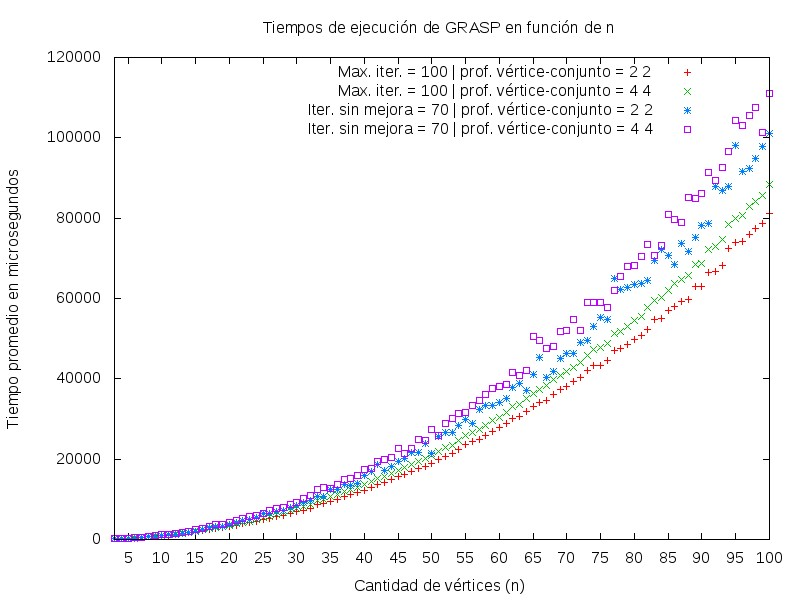
\includegraphics[width=\textwidth]{ejercicio-5-tiempos-grasp-conjunto-1.jpg}}
		\label{fig:ejercicio-5-tiempos-grasp-conjunto-1}
    \end{minipage}
\end{figure}

Vemos por un lado que a mayor $n$, el criterio de iteraciones sin mejora con ambas profundidades toma más tiempo que el criterio de iteraciones máximas, y que para cada una de ellas, usar más profundidad lleva también más tiempo. Lo primero lo explicamos con nuestra hipótesis: iteraciones sin mejora hace más iteraciones que el máximo a mayor $n$, y esta es una de las razones por las que termina dando mejores soluciones. Por otro lado, usar más profundidad hace que la golosa aleatorizada provea soluciones más distantes, y que haya más probabilidad de que la búsqueda local las mejore para superar a la mejor partición hasta el momento. Esto sugiere que usar más profundidad genera mejores soluciones. Falta ver qué ocurre para los primeros $n$:

\begin{figure}[H]
    \begin{minipage}[t]{\linewidth}
		\centering
		\frame{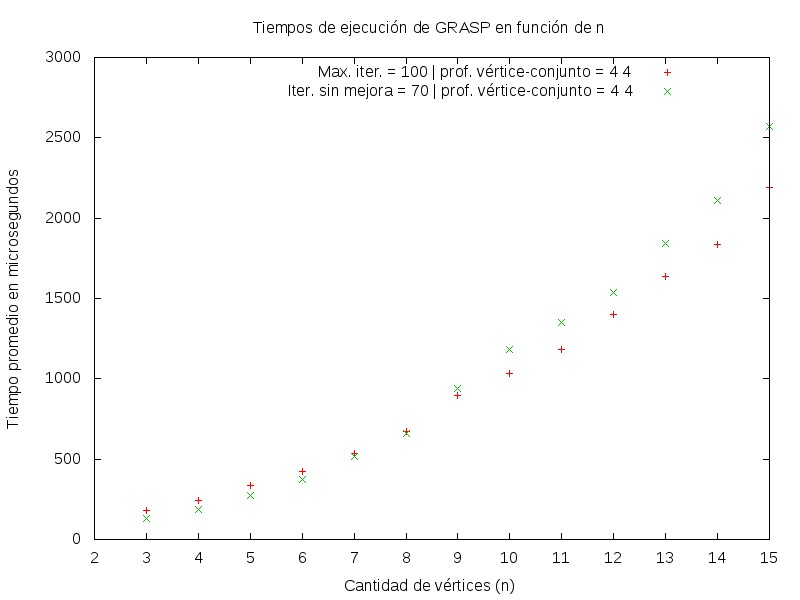
\includegraphics[width=\textwidth]{ejercicio-5-tiempos-grasp-primeros-nodos-conjunto-1.jpg}}
		\label{fig:ejercicio-5-tiempos-grasp-primeros-nodos-conjunto-1}
    \end{minipage}
\end{figure}

Como preveíamos, para grafos pequeños termina antes usar iteraciones sin mejora, aunque rápidamente iteraciones sin mejora comienza a superar las 100 iteraciones, y por esto es mayor para $n \geq 9$. La razón por la cual la diferencia es poco apreciable es que estamos usando como límite de iteraciones sin mejora a 70, pero ya vimos en el test de configuración que para valores menores a 15 podríamos usar 10, 35 ó 50 y así ---sin perder calidad--- obtener mayores diferencias en el tiempo de ejecución.

\section{Experimentación} 

\noindent En este momento contamos con varios algoritmos para resolver el problema de $k$-PMP:
\begin{enumerate}
  \item Algoritmo exacto.
  \item Algoritmo goloso.
  \item Heurísticas de búsqueda local y sus respectivas vecindades \textbf{(a)} swap y \textbf{(b)} jump.
  \item GRASP.
\end{enumerate}

El único de ellos que nos garantiza que la solución obtenida es óptima, exacta en este caso, es el algoritmo exacto.
El resto no exploran todo el espacio de soluciones sino que intentan recorrer un subconjunto acotado del mismo,
guiados por alguna heurística, y extraer la mejor del subconjunto explorado. El algoritmo exacto y el goloso
no requieren de configuración alguna, en cambio la búsqueda local y el GRASP sí requieren configuración y por lo tanto
dependiendo de la configuración que se utilice pueden devolver resultados diferentes para la misma instancia.
% recordar cuáles fueron las mejores configuraciones obtenidas para los configurables
Por esta razón, en sus respectivas secciones, nos dedicamos a analizar cuáles eran las mejores configuraciones.
Finalmente obtuvimos:

\begin{description}
  \item[búsqueda local] la vecindad \textit{jump} se mostró superior tanto en calidad como en tiempos de ejecución.
  \item[GRASP] profundidad de la elección de vértices 4 y profundidad de elección de conjuntos 4. 
\end{description}

% presentar el objetivo de la experimentación
El objetivo de la siguiente experimentación es comparar la performance de los algoritmos en función de la calidad de las soluciones obtenidas y de la performance en términos de tiempos de ejecución. Para ello
generamos un nuevo conjunto de instancias, diferente al conjunto con el cual fueron entrenadas, es decir
con el cual realizamos las experimentaciones para conseguir las mejores configuraciones. El conjunto de
instancias con el cual cada uno de los algoritmos fue entrenado no es necesariamente representativo, con
esto queremos decir que si bien obtuvimos una configuración superior en ese conjunto de instancias, esa
configuración no será necesariamente superior en otro conjunto de instancias o en 
familias particulares de grafos (instancias). Un claro ejemplo de esto es la familia de instancias
patológicas que describimos para el algoritmo goloso.
% aclarar cómo fue generado el nuevo conjunto de instancias
El conjunto de instancias fue generado de la misma manera que el que utilizamos para los tests de configuración
de GRASP. Al ser pseudoaleatorios con mínimas restricciones, como por ejemplo sobre la densidad mínima para que
las instancias no sean triviales, son independientes de dicho conjunto.

\subsection{Tiempos de ejecución}
% explicar que los tiempos del exacto sólo están hasta el 23 inclusive
En primer lugar, compararemos los tiempos de ejecución de los algoritmos tomando el promedio
sobre 100 instancias con una misma cantidad de vértices. El algoritmo exacto sólo
aparece graficado hasta $n=23$ porque para valores mayores toma demasiado tiempo.
% describir nuestras estimaciones
Nosotros estimamos que el exacto será el más lento por varios órdenes de magnitud y luego
vendrán GRASP, el goloso con la búsqueda local y por último el goloso sin búsqueda local. Creemos que será así
porque en cierta forma unos están incluidos en los otros. GRASP ejecuta un goloso aleatorizados
varias veces y a cada uno le aplica la heurística de búsqueda local, por lo cual en términos
de costos realiza el mismo trabajo que la heurística de búsqueda local pero muchas veces.
El goloso con la heurística de búqueda local primer ejecuta el goloso, por lo cual su costo
es el del goloso más el costo de la heurística de búsqueda local.

% gráficos
% explicar por qué creemos que es más ilustrativo presentar los mismos valores pero en distintos gráficos
\begin{figure}[H]
    \begin{minipage}[t]{\linewidth}
		\centering
		\frame{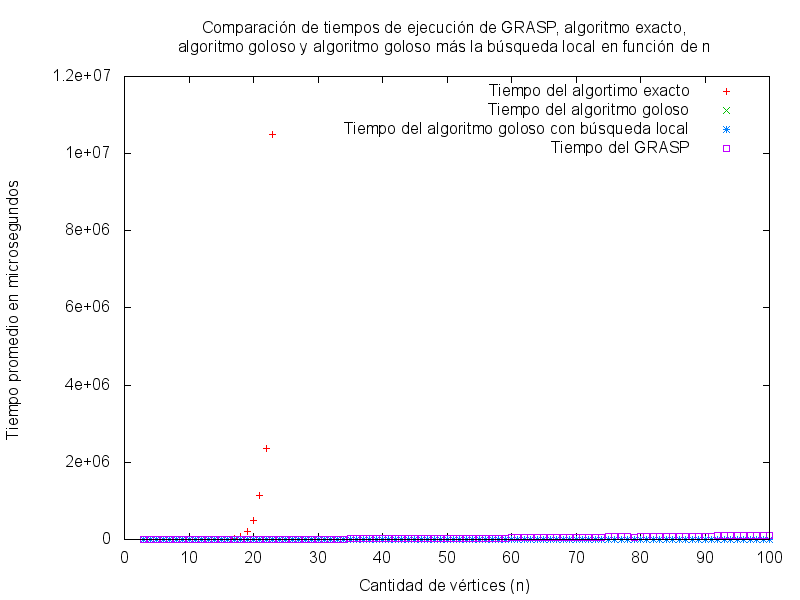
\includegraphics[width=\textwidth]{ejercicio-6-comparacion-tiempos.png}}
		\label{fig:ejercicio-6-comparacion-tiempos}
    \end{minipage}
\end{figure}
A partir de $n=19$ los tiempos del algoritmo exacto se vuelven muy grandes y se puede apreciar
que el crecimiento parece ser mucho mayor que exponencial. En comparación con los tiempos del exacto
el resto de los algoritmos parecen constantes, es por esto que decidimos graficar los mismos valores 
pero sin los tiempos del exacto para poder apreciar mejor sus diferencias y tendencias de crecimiento.
\begin{figure}[H]
    \begin{minipage}[t]{\linewidth}
		\centering
		\frame{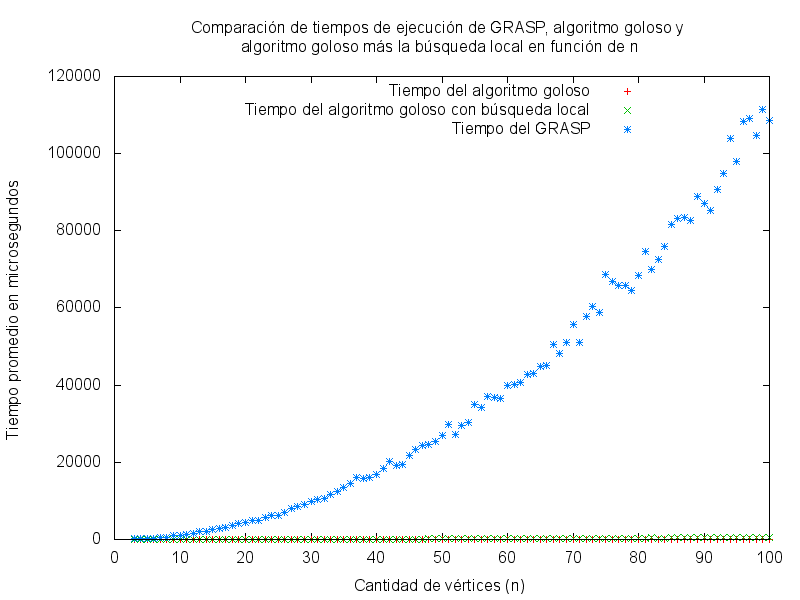
\includegraphics[width=\textwidth]{ejercicio-6-tiempos-menos-exacto.png}}
		\label{fig:ejercicio-6-comparacion-tiempos-menos-exacto}
    \end{minipage}
\end{figure}
Una vez más uno de los algoritmos tuvo tiempos de ejecución muy superiores al resto, en este caso fue GRASP.
Sin embargo, el crecimiento de GRASP se muestra mucho más suave que el presentado por el exacto en el gráfico anterior.
Como no se puede apreciar la diferencia entre el goloso con y sin búsqueda local decidimos graficarlos por separado
ya que comparándolos con GRASP parecen constantes.
\begin{figure}[H]
    \begin{minipage}[t]{\linewidth}
		\centering
		\frame{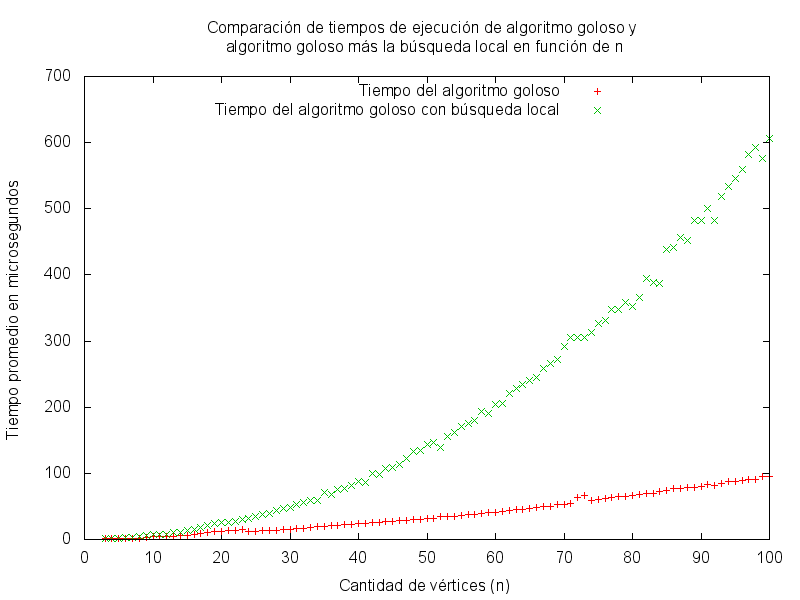
\includegraphics[width=\textwidth]{ejercicio-6-tiempos-menos-grasp.png}}
		\label{fig:ejercicio-6-comparacion-tiempos-menos-grasp}
    \end{minipage}
\end{figure}
Finalmente podemos apreciar la diferencia entre el goloso con y sin la búsqueda local. Vemos
que la búsqueda local no agrega sólo una constante al crecimiento del goloso, mas bien aumenta por
lo menos en $n$ su costo ya que  el goloso parece lineal y el goloso con la búsqueda local al menos cuadrático.
% análisis de los gráficos
El orden de méritos no presentó sorpresas pero los gráficos sí nos dejaron apreciar las diferencias entre 
uno y el siguiente. Podemos concluir que los tiempos de ejecución son órdenes de magnitud superiores entre
uno y otro algoritmo. El exacto presenta tiempos inutilizables en la práctica. GRASP tiene un performance
mucho mejor, la cual permite su utilización en la práctica, pero su costo es muy superior al del goloso con o sin búsqueda local.
Ahora necesitamos analizar la calidad de las soluciones que cada uno consigue para saber si el costo
temporal que implica GRASP redunda en una mejor calidad de sus soluciones o no.

\subsection{Calidad de las soluciones}
% describir nuestras estimaciones
Creemos que la calidad de las soluciones van a seguir el mismo orden que los tiempos de ejecución
principalmente por la inclusión de unos algoritmos en otros como ya explicamos en la sección anterior.
Creemos que la calidad de GRASP no va llegar a ser igual a la del exacto pero esperamos
que esté mucho más cerca que el goloso con y sin búsqueda local. Creemos que los dos mayores saltos
estarán entre el exacto y el GRASP y entre GRASP y los golosos.
% explicar que la calidad del exacto sólo está hasta el 23 inclusive
Decidimos primero graficar sólo con $n < 24$, los valores que alcanza el exacto, para poder apreciar
mejor las diferencias en este rango en el que contamos con la respuesta exacta.
% gráficos
\begin{figure}[H]
    \begin{minipage}[t]{\linewidth}
		\centering
		\frame{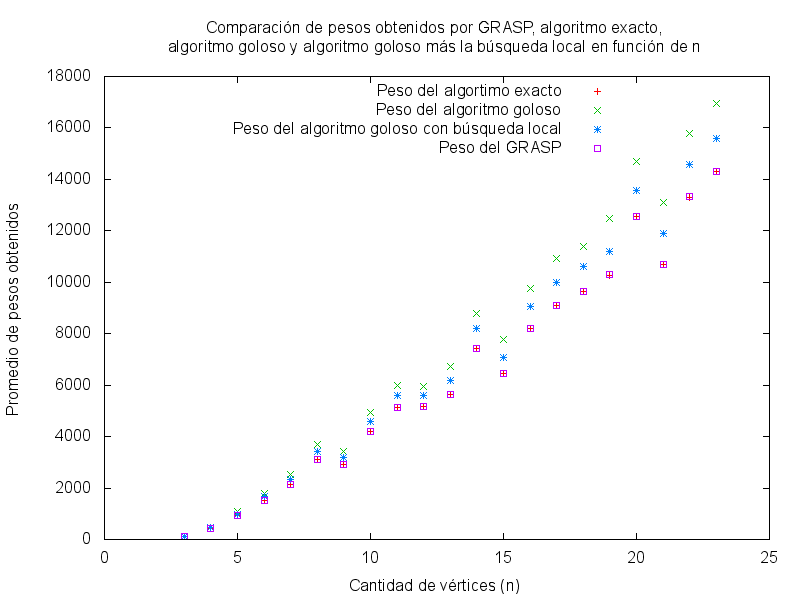
\includegraphics[width=\textwidth]{ejercicio-6-comparacion-calidad.png}}
		\label{fig:ejercicio-6-comparacion-calidad}
    \end{minipage}
\end{figure}

Sorprendentemente podemos ver que GRASP, al menos para éste rango de valores, tiene una calidad
igual que la del exacto. El orden es el que esperábamos pero no así la diferencia entre uno y el otro.
Sin embargo, parece que la tendencia es que la diferencia entre GRASP y goloso con búsqueda local, y
entre goloso con y sin búsqueda local, aumente junto con $n$.

\begin{figure}[H]
    \begin{minipage}[t]{\linewidth}
		\centering
		\frame{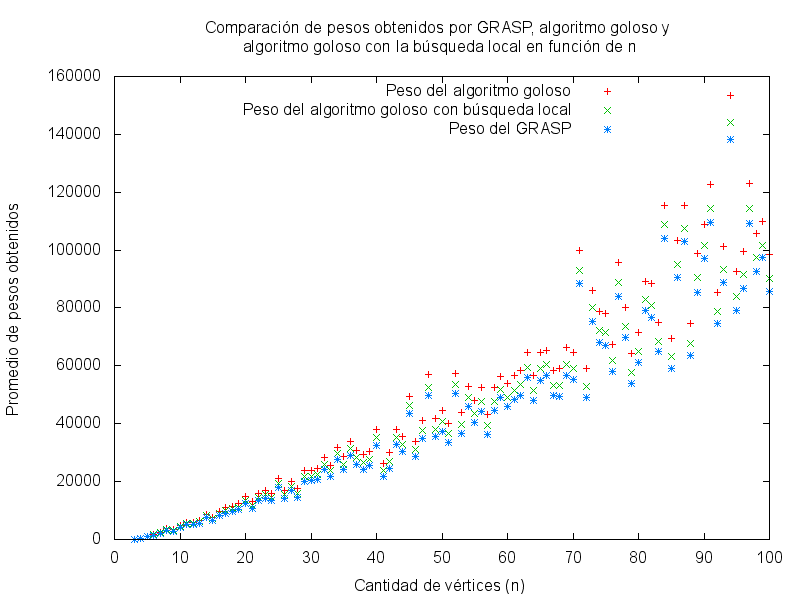
\includegraphics[width=\textwidth]{ejercicio-6-comparacion-calidad-sin-exacto.png}}
		\label{fig:ejercicio-6-comparacion-calidad-sin-exacto}
    \end{minipage}
\end{figure}

En este gráfico podemos ver que la diferencia entre GRASP y el goloso con búqueda local
parece no aumentar significativamente, si bien GRASP siempre consigue mejores resultados. La
diferencia entre goloso con búsqueda local y sin búsqueda local sí parece aumentar pero no queda
claro.
Finalmente decidimos graficar el error relativo presentado por todos los algoritmos con respecto al
exacto en el rango permitido. Este gráfico creemos que dará una idea más clara acerca de la distancia
entre la calidad de las soluciones de uno y otro algoritmo.

\begin{figure}[H]
    \begin{minipage}[t]{\linewidth}
		\centering
		\frame{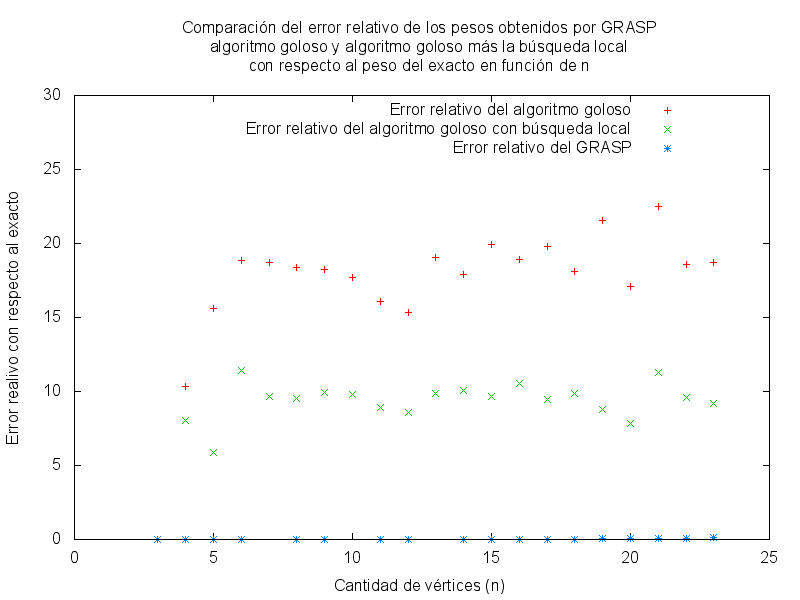
\includegraphics[width=\textwidth]{ejercicio-6-comparacion-calidad-error-relativo.png}}
		\label{fig:ejercicio-6-comparacion-calidad-error-relativo}
    \end{minipage}
\end{figure}

Se ve que el goloso con búsqueda local parece ubicarse generalmente apenas por debajo del $10\%$ y 
el goloso sin búsqueda local alrededor del $20\%$. La diferencia entre cada uno parece mostrar
un salto de aproximadamente $10\%$ de calidad entre uno y otro algoritmo. Si tuviéramos algún 
contexto particular éstas diferencias puede que cambien rotundamente.
% análisis de los gráficos

Pudimos ver que el costo temporal superior presentado por GRASP redunda en una mejor calidad, 
sin embargo, no queda claro que la ganancia sea muy grande, es decir parece que los tiempos
de ejecución son mucho mayores que la ganancia obtenida en la calidad de las soluciones. Ésto
claramente depende del contexto ya que ---por ejemplo--- el salto de $10\%$ que aproximamos de los
resultados obtenidos, en ciertos contextos puede ser una gran diferencia.


%\section{Conclusiones}
%
%Discutimos sobre criterios de parada y sobre la selección de candidatos de la golosa aleatorizada, y elegimos una configuración en base a los resultados obtenidos para un primer conjunto de instancias.
%
%Testeamos sobre dos criterios de parada y comentamos sus beneficios y problemas. En una aplicación real, sería conveniente por lo menos usar una combinación de ambos criterios, es decir, iteraciones sin mejora pero con un límite máximo de iteraciones global. Por otro lado, para distintos valores de $n$, vimos que es conveniente variar los límites para reducir el tiempo de ejecución, por lo cual sería interesante tener límites dinámicos según la cantidad de vértices del grafo de entrada.
%
%Para la selección de candidatos de la golosa aleatorizada, testeamos varios niveles de profundidad de elección de vértice y de elección de conjunto. No fue claro en particular que la mejor profundidad sea $(4,4)$, ya que aunque resultó ganadora, los errores relativos eran tan cercanos a cero que bien podría tratarse de una acumulación de los errores de cálculo inherentes a la aritmética finita. Sí es más claro que es más importante aleatorizar la elección del conjunto destino.
%
%Elegimos la configuración de iteraciones sin mejora y profundidad de elección de vértice-conjunto $(4,4)$ y comparamos los resultados del primer conjunto con un nuevo conjunto de iteraciones. Vimos que aunque los tiempos de ejecución se mantuvieron intactos, la calidad no fue la esperada, teniendo en algunos casos el doble de error relativo para el segundo conjunto. Esto sugiere que no hay garantía de que una configuración funcione relativamente bien siempre, la única garantía de calidad parece ser la cantidad de iteraciones que realiza la GRASP.

\newpage
\section{Apéndice}

\newpage
% Bibliografía
%\addcontentsline{toc}{section}{Referencias}
\begin{thebibliography}{11}

\bibitem{cormen}
  Thomas H. Cormen,
  \emph{Introduction to Algorithms}.
  The MIT Press, Massachusetts,
  3rd edition,
  2009.

\end{thebibliography}
%\bibliographystyle{plain}
%\bibliography{referencias}

\end{document}
